%\RequirePackage{lineno}
\documentclass[12pt,a4paper,twoside,titlepage,final,openany]{book}


%% ---- style files ------
\usepackage{bstyle}
%\author{B. MOUGINOT \& B. LENIAU}
%\title{CLASS Userguide.}
%
%\date\today



%----------------------------------------------------------------------------------------
%	BLANK DOCUMENT
%----------------------------------------------------------------------------------------


%% --------- MAIN -------------
\begin{document}
\titleGM % This command includes the title page
% === title and abst. ===
\pagestyle{empty}
%\include{abstract}
\frontmatter
\phantomsection
%\addcontentsline{toc}{part}{Abstract}
%\chapter*{{\large Abstract}}
\clearpage
\phantomsection
\addcontentsline{toc}{part}{Table of Contents}
\tableofcontents
%
\clearpage
\phantomsection
\addcontentsline{toc}{part}{List of figures}
\listoffigures


%%%%%%%%%%%%%%%%%%%%%%%%%
%% CHAPTER :	INTRODUCTION
%%%%%%%%%%%%%%%%%%%%%%%%%
\mainmatter
% !TEX root = USEGUIDE.tex
\pagenumbering{arabic}


\part{Introduction}

    \begin{figure}[H]
    \centering
    \centerline{
\includegraphics[scale=0.2]{LOGO_CLASS.png}}
    \caption{CLASS logo}
    \label{fig:CLASSLogo}
    \end{figure}

    \vspace{2cm}

The code CLASS (\textbf{C}ore \textbf{L}ibrary for \textbf{A}dvanced \textbf{S}cenario \textbf{S}imulation) is a dynamic fuel cycle simulation tool developed by CNRS/IN2P3 (Centre National de la Recherche Scientifique / Institut National de Physique Nucléaire et de Physique des Particules) in collaboration with IRSN (Institut de Radioprotection et de Sûreté Nucléaire). The aim of the tool CLASS is to model an evolving electro-nuclear fleet. The main output is the evolution of isotopes in all facilities of a nuclear fleet. The reactor physics is located in the treatment of the fuel fabrication and its depletion in reactor. The code CLASS aims to be a useful tool for scenarios studies. CLASS main asset is its ability to implement any kind of reactor, either the system is innovative or standard. Indeed, the opportunity is given to each user to \textbf{build his own reactor model}.

\part{First Steps}
\chapter{Package Content}
The CLASS package contains the followings :
\begin{itemize}
\item   \textbf{data/} : folder containing nuclei properties
\subitem \textbf{FPyield\_Fast\_JEFF3.1.dat }     : file containing fission yield for fast reactors
\subitem \textbf{FPyield\_Thermal\_JEFF3.1.dat}   : file containing fission yield for thermal reactors
\subitem \textbf{Mass.dat }                     : file containing molar masses
\subitem \textbf{SpontaneousFPyield.dat }       : file containing spontaneous fission yields
\subitem \textbf{chart.JEF3T}                   : file containing decay constants and branching ratios
\subitem \textbf{HeatTox.dat}                   : file containing conversion data for heat and radiotoxicity calculation

 \item \textbf{DATA\_BASES/}  : this folder contains decay data base and reactor data bases
 \subitem \textbf{DECAY/}     : decay data base
 \subitem \textbf{FBR-Na/}    : Models related to Fast reactor
 \subitem \textbf{PWR/}       : Models related to Pressurised Water Reactor
 \subitem \textbf{REP\_HFC/}   : Models related to low moderated Pressurised Water Reactor 
 \subitem \textbf{ADS/}       : Models related to Accelerator Driven System
 
 \item \textbf{documentation/} 
 \subitem \textbf{Manual/}    : folder containing this user guide an its .tex sources
 \subitem \textbf{Doxygen/}   : folder containing the builded doxygen and its generation configuration 

\item \textbf{example/} : folder containing simple examples of CLASS input and an example of CLASS ouput reader

\item \textbf{gui/} : folder containing sources of the graphical user interface for CLASS outputs
 
\item \textbf{lib/} : folder containing the CLASS library (once compiled)
\item \textbf{bin/} : folder containing the CLASSGui and the Google test binary (once compiled)

\item \textbf{source/} : folder containing CLASS sources
\subitem \textbf{include/}
\subitem \textbf{Model/} : folder that contain the sources related to the physics models (EquivalenceModel , XSModel and IrradiationModel)
\subitem \textbf{src/}
\subitem \textbf{External/} : folder that contain the sources related to external classes used by the code CLASS

\item \textbf{Utils/} : folder containing utility software related to reactor data base generation
\subitem \textbf{EQM/} : Example of software to generate equivalence model for building reactor fuel
\subitem \textbf{MURE2CLASS/} : Software to convert MURE (a fuel depletion code)  output to \hyperref[sec:EvolutionData]{EvolutionData} format
\subitem \textbf{XSM/} : Software to generate cross section predictor
\subitem \textbf{ROOT2DAT/} : Software to convert CLASS output into readable ASCII data file
\subitem \textbf{ROOT2ROOT/} : Software to convert multiple CLASS Output into one single ROOT file (used for sensitivity analysis)
 
 
\end{itemize}

\chapter{Install procedure}

\section{Requirement}

\begin{itemize}
\item User skills : Good knowledge of C++. Abilities in using \href{https://root.cern.ch/}{Root}\footnote{https://root.cern.ch/}.
Experience in depletion codes and neutron transport codes is required for building complex new reactor model.
\item OS : CLASS is known to work under Linux (64  bits) and MacOSX (64 bits). It  has never been tested on any Windows distribution.
\item C++ compiler :  we recommend to use a gnu compiler like gcc4.8 or above. For OSX, CLASS is working with native clang compiler.
\item For DARWIN (OSX) users : 
Make sure you have installed XCode and its command line tools (if not dowload and install from AppStore). If using clang compiler, there's no possibility to use openmp. 
\item Root (CERN) :  
ROOT~\cite{Brun_1997} is an analysis software developped by CERN. CLASS version 5 uses some ROOT version 6 features to run. CLASS uses Root to store output data. The graphical user interface CLASSGui is also based on Root. Some algorithms uses the TMVA module of Root. 
\end{itemize}

\section{Installation}
Decompress the CLASS.tar.gz in your wanted location. 

 Then type in terminal:
\begin{center}
\begin{minipage}{\textwidth}
\begin{lstlisting}[style=terminal]
cd < CLASS root folder >
./install.sh --help
\end{lstlisting}
\end{minipage}
\end{center}

You should have in terminal the help of CLASS install script :
\begin{center}
\begin{minipage}{\textwidth}
\begin{lstlisting}[style=terminal]
###############################################################
############## configures and compiles CLASS V4.1 #############
###############################################################

Usage: install.sh [VAR=VALUE] [OPTION]
Defaults for the options are specified in brackets.

Configuration:
  -h, --help         display this help and exit
Optional Features:
  --disable-OMP      do not compile with OpenMP support for evolution 
                     [default: enable for gcc version >= 4.1]
  --InstallLib-path=path     Location of made CLASS's libraries [default= $PWD/lib]

Some influential environment variables:
  CXX         C++ compiler command [default=g++]
  CXXFLAGS    C++ compiler flags, e.g. -I<include dir> if
              you have headers in a nonstandard directory <include dir>
  CPPFLAGS    C++ preprocessor flags, e.g. -D<special flag>

Report bugs to <leniau@subatech.in2p3.fr>.
(special thanks to PTO)
\end{lstlisting}
\end{minipage}
\end{center}
We suggest to use the default install by typing :
\begin{center}
\begin{minipage}{\textwidth}
\begin{lstlisting}[style=terminal]
./install.sh
\end{lstlisting}
\end{minipage}
\end{center}
This script (used without argument) will compile and install CLASS libraries in < CLASS root folder >/lib.
It will build CLASSGui binary in < CLASS root folder >/gui/bin/.It will set the correct pathway for the decay data base and add the CLASS environment variables in your \$HOME/.(shell)rc. With (shell) is your default shell. If everything goes well, you should see in terminal something like (see next page) and be able to compile your first CLASS input:
\begin{center}
\begin{minipage}{\textwidth}
\begin{lstlisting}[style=terminal]
Checking for ROOT cern lib... yes
Checking for omp.h... yes
   You can disable the use of this library with "--disable-OMP" option
Building Librairies Folder @ /scratch/leniau/App/local/CLASS_Support/lib
####################################################
######### Compilation of CLASS libraries ###########
####################################################
[...]
libCLASSpkg.so done
[...]
libCLASSpkg_root.so done
####################################################
########## Compilation Done  #######################
####################################################
MURE libraries installed in
----> /scratch/leniau/App/local/CLASS_Support/lib
####################################################
######### Compilation of CLASSGUI binary ###########
####################################################
[...]
CLASSGui is now available in /scratch/leniau/App/local/CLASS_Support/gui/bin 
####################################################
########## Compilation Done  #######################
####################################################
####################################################
########## SET DECAY DATA BASES PATHES #############
####################################################
-> Done
/scratch/leniau/App/local/CLASS_Support
####################################################
########## ENVIRONEMENT VARIABLES ##################
####################################################
-> Your default shell is : /bin/tcsh
-> Your .tcshrc will be edited if CLASS_PATH CLASS_include
   and CLASS_lib aren't defined yet 

CHECKING LOADED ENVIRONEMENT VARIABLES ............
Not found in your loaded .tcshrc. 
Setting variables ...

PRESS ENTER IF DEFAULT IS CORRECT
====>ENTER THE PATH TO THE CLASS root folder (defalut /scratch/leniau/App/local/CLASS_Support) 
Path of the CLASS include folder is /scratch/leniau/App/local/CLASS_Support

====>ENTER THE PATH TO THE CLASS INCLUDE (default: /scratch/leniau/App/local/CLASS_Support/source/include/): 
Path of the CLASS include folder is /scratch/leniau/App/local/CLASS_Support/source/include/

====>ENTER THE PATH WHERE CLASS LIB ARE INSTALLED (default: /scratch/leniau/App/local/CLASS_Support/lib): 
Path of the CLASS lib folder is /scratch/leniau/App/local/CLASS_Support/lib

Environnment variables added in /Users/leniau/.tcshrc
LOADING /Users/leniau/.tcshrc ... done

!!!!!!!!!!!!!!!!!!!!!!!!!!!!!!!!!!!!!!!!!!!!!!!!!!!!!!!!!!!!
 Congratulations you are now able to compile your first     
               CLASS .cxx input.                            
 Please read /scratch/leniau/App/local/CLASS_Support/documentation/Manual/USEGUIDE.pdf
 !!!!!!!!!!!!!!!!!!!!!!!!!!!!!!!!!!!!!!!!!!!!!!!!!!!!!!!!!!!!
\end{lstlisting}
\end{minipage}
\end{center}

Please report installation issues to the \href{https://forge.in2p3.fr/projects/classforge/issues/new}{forge}\footnote{https://forge.in2p3.fr/projects/classforge/issues/new}.

\chapter{CLASS Execution}
CLASS is a set of C++ libraries, there is no CLASS binary file. A CLASS executable has to be build by user using objects and methods defined in the CLASS package. \\
The compilation line for generating your executable from a .cxx file is the following :
(You can find CLASS input examples in \$CLASS\_PATH/example/)

\begin{center}
\begin{minipage}{\textwidth}
\begin{lstlisting}[style=terminal]
g++ -o CLASS_exec YourScenario.cxx -I $CLASS_include -L $CLASS_lib -lCLASSpkg `root-config --cflags` `root-config --libs` -fopenmp -lgomp -Wunused-result -lTMVA
\end{lstlisting}
\end{minipage}
\end{center}
Then type 
\begin{center}
\begin{minipage}{\textwidth}
\begin{lstlisting}[style=terminal]
./CLASS_exec
\end{lstlisting}
\end{minipage}
\end{center}

The following should show in your terminal :

    \begin{figure}[H]
    \centering
    \centerline{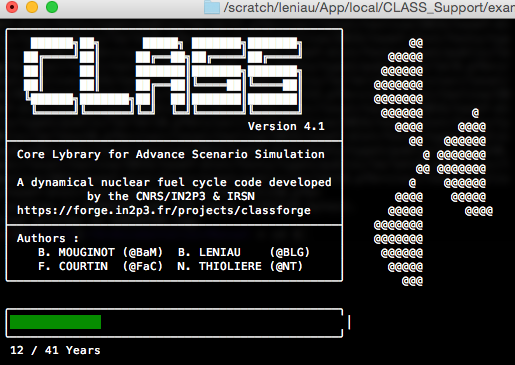
\includegraphics[scale=0.9]{CLASS_Run.png}}
    \caption{CLASS running in a shell}
    \label{fig:CLASSRUN}
    \end{figure}




\chapter{News, forum, troubleshooting, doxygen ...}
CLASS has a \href{https://forge.in2p3.fr/projects/classforge}{forge}\footnote{https://forge.in2p3.fr/projects/classforge} hosted by the IN2P3  where you can find :

\begin{itemize}
\item \href{https://forge.in2p3.fr/projects/classforge/boards}{A forum}\footnote{https://forge.in2p3.fr/projects/classforge/boards} where you are invited to post your trouble about CLASS installation and usage. You may find the answer to your trouble on a already posted thread.
\item \href{https://forge.in2p3.fr/projects/classforge/embedded/doxygen/inherits.html}{A doxygen}\footnote{https://forge.in2p3.fr/projects/classforge/embedded/doxygen/inherits.html} where all the CLASS objects and methods are defined and explained. Note that the doxygen is also contained in \$CLASS\_PATH/documentation/doxygen/CLASSDoxygen.html
\item \href{https://forge.in2p3.fr/projects/classforge/news}{News}\footnote{https://forge.in2p3.fr/projects/classforge/news} : All the news related to CLASS
\end{itemize}
A \href{classuser-l@ccpntc02.in2p3.fr}{Mailing List}\footnote{classuser-l@ccpntc02.in2p3.fr} also exist in order to be warned of all the change inside CLASS and to allow user to exchange directly on the code. One can join the mailing list through the following  \href{http://listserv.in2p3.fr/cgi-bin/wa?SUBED1=classuser-l&A=1}{link}\footnote{http://listserv.in2p3.fr/cgi-bin/wa?SUBED1=classuser-l\&A=1}.





%%%%%%%%%%%%%%%%%%%%%%%%%
%% CHAPTER :	GENERAL OVERVIEW
%%%%%%%%%%%%%%%%%%%%%%%%%
% !TEX root = USEGUIDE.tex

\part{CLASS : General overview}
\chapter{Generalities}
\section{Basic unit\label{sec:cSecond}}
All time in CLASS should be written in second. It corresponds to the cSecond, a CLASS c++ type, which are a \textbf{long long int} going, in 32 bits \textbf{and} 64 bits, up to  $(2^{63} - 1)~\textrm{s}~ \sim 2.9\cdot 10^{11}$ years, enough for any electro-nuclear scenarios one can consider....\\
 \section{CLASS working process principle}
image : sh�ma de principe de class
\chapter{Facilities descriptions}
All the facilities in CLASS project are regrouped inside a large group called CLASSFacility (and inherit of all the properties of the CLASSFacility in a C++ way). Inside the CLASSFacility, 3 different types has been defined, the reactor, the FabricationPlant (or more generally, all the fuel cycle front-end facilities) and the backend facilities. 
\section{CLASSFacility\label{sec:CLASSFacility}}
The CLASSFacility should never be used directly in the main CLASS program (the one made to perform the simulation).  The aim of these object is to regroup all the common properties of the nuclear facilities, such as common variables, methods, and builder. 


\section{Reactor\label{sec:reactor}}
\subsection{Generalities}
The aim of this class is to deal with the evolution of the fuel inside a reactor.\\
The evolution of the fuel is \textbf{always} contain in the \hyperref[sec:EvolutionData]{EvolutionData} \textit{fEvolutionDB}.\\
There are 2 way to provide the \hyperref[sec:EvolutionData]{EvolutionData} to the reactor. In the case of fixed fuel\footnote{Always the same input/output isotopic composition.} the user need to provide it, using the appropriated constructor, the set function, or a \hyperref[sec:CLASSFuelPlan]{CLASSFuelPlan}. In the case of recycled fuel or unfixed fuel, the user need to provide a \hyperref[sec:PhysicsModels]{PhysicsModels}, using the appropriated constructor, the set function, and/or a \hyperref[sec:CLASSFuelPlan]{CLASSFuelPlan}.

\subsection{Use}
There are 2 main ways to define a reactor, depending on the type of fuel loaded.

\subsubsection{Fixed Fuel}
Reactor using fixed fuel, which load always the same fresh fuel, and unload it with always the same burnup (same spent fuel...), to declare a reactor proceed as follow:
\begin{center}
\begin{minipage}{\textwidth}
\begin{lstlisting}
Reactor *MyReactor = new reactor(aCLASSLogger,		// CLASSLogger
				 myFuel_EvolutionData,	// EvolutionData
				 aBackEnd,		// BackEnd
				 myRe_StartingTime,	// Starting Time
				 myRe_LifeTime,		// Time of Life
				 myRe_Power,		// Power
				 myRe_HeavyMetalMass,	// HM mass
				 myRe_BurnUp,		// BurnUp
				 myRe_LoadFactor);	// LoadFactor
\end{lstlisting}
\end{minipage}
\end{center}
or
\begin{center}
\begin{minipage}{\textwidth}
\begin{lstlisting}
Reactor *MyReactor = new reactor(aCLASSLogger,		// CLASSLogger
				 myFuel_EvolutionData,	// EvolutionData
				 aBackEnd,		// BackEnd
				 myRe_StartingTime,	// Starting Time
				 myRe_LifeTime,		// Time of Life
				 myRe_CycleTime,	// Time of Cycle
				 myRe_HeavyMetalMass,	// HM mass
				 myRe_BurnUp);		// BurnUp
\end{lstlisting}
\end{minipage}
\end{center}
The meaning of each arguments of the two constructor previously defined are summed up in the following table

\begin{table}[H]
\begin{center}
\caption{Arguments of Reactor constructors}
\label{tab:meanKeyWord}
\begin{tabular}{|c|c|c|c|}
\hline
Argument & type & meaning & unit \\
\hline
aCLASSLogger 		&	\hyperref[sec:CLASSLogger]{CLASSLogger}		& Output messages 			& N.A.\\
myFuel\_EvolutionData	&	\hyperref[sec:EvolutionData]{EvolutionData}	& Fuel evolution description		& N.A. \\
aBackEnd 		&	\hyperref[sec:CLASSBackEnd]{CLASSBackEnd}	& Facility getting the spent fuel 	& N.A. \\
myRe\_StartingTime 	&	\hyperref[sec:cSecond]{cSecond}			& Creation time 			& second\\
myRe\_LifeTime 		&	\hyperref[sec:cSecond]{cSecond}			& Operation time 			& second\\
myRe\_Power 		&	double						& Thermal power 			& Watt\\
myRe\_HeavyMetalMass 	&	double						& Heavy metal mass 			& tons\\
myRe\_BurnUp 		&	double						& Burn up at EOC 			& GWd/tHM\\
myRe\_LoadFactor 	&	double						& Fraction of nominal power 		& .\\
myRe\_CycleTime 	&	\hyperref[sec:cSecond]{cSecond}			& the cycle time 			& second\\
\hline
\end{tabular}
\end{center}
\end{table}


\subsubsection{Reprocessed Fuel}
In this case, the fuel is provided by an external facility, so called, the \hyperref[sec:FabricationPlant]{FabricationPlant}. The way to build the reprocessed fresh fuel and to handle the fuel depletion calculation is done by the \hyperref[sec:PhysicsModels]{PhysicsModels}.
The main ways to defined a Reactor (with reprocessed fuel) is shown in the next two examples :

\begin{center}
\begin{minipage}{\textwidth}
\begin{lstlisting}
Reactor *MyReactor = new Reactor(aCLASSLogger,		// CLASSLogger
				 myFuel_PhysicsModels,	// PhysicsModels
				 aFabricationPlant,	// FabricationPlant
				 aBackEnd,		// BackEnd
				 myRe_StartingTime,	// Starting Time
				 myRe_LifeTime,		// Time of Life
				 myRe_Power,		// Power
				 myRe_HeavyMetalMass,	// HM mass
				 myRe_BurnUp,		// BurnUp
				 myRe_LoadFactor);	// LoadFactor
\end{lstlisting}
\end{minipage}
\end{center}
or
\begin{center}
\begin{minipage}{\textwidth}
\begin{lstlisting}
Reactor *MyReactor = new Reactor(aCLASSLogger,		// CLASSLogger
				 myFuel_PhysicsModels,	// PhysicsModels
				 aFabricationPlant,	// FabricationPlant
				 aBackEnd,		// BackEnd
				 myRe_StartingTime,	// Starting Time
				 myRe_LifeTime,		// Time of Life
				 myRe_CycleTime,	// Time of Cycle
				 myRe_HeavyMetalMass,	// HM mass
				 myRe_BurnUp);		// BurnUp
\end{lstlisting}
\end{minipage}
\end{center}
The meaning of each arguments of the two constructor previously defined are summed up in the following table

\begin{table}[H]
\begin{center}
\caption{Arguments of Reactor constructors}
\label{tab:meanKeyWord}
\begin{tabular}{|c|c|c|c|}
\hline
Argument & type & meaning & unit \\
\hline
aCLASSLogger 		& \hyperref[sec:CLASSLogger]{CLASSLogger}		& Output messages 			& N.A.\\
myFuel\_PhysicsModels	& \hyperref[sec:PhysicsModels]{PhysicsModels}		& Fuel construction/evolution		& N.A. \\
aFabricationPlant 	& \hyperref[sec:FabricationPlant]{FabricationPlant}	& Facility building the fuel 		& N.A. \\
aBackEnd 		& \hyperref[sec:CLASSBackEnd]{CLASSBackEnd}		& Facility getting the spent fuel 	& N.A. \\
myRe\_StartingTime 	& \hyperref[sec:cSecond]{cSecond}			& Creation time 			& second\\
myRe\_LifeTime 		& \hyperref[sec:cSecond]{cSecond}			& Operation time 			& second\\
myRe\_Power 		& double						& Thermal power 			& Watt\\
myRe\_HeavyMetalMass 	& double						& Heavy metal mass 			& tons\\
myRe\_BurnUp 		& double						& Burn up at EOC 			& GWd/tHM\\
myRe\_LoadFactor 	& double						& Fraction of nominal power 		& .\\
myRe\_CycleTime 	& \hyperref[sec:cSecond]{cSecond}			& the cycle time 			& second\\
\hline
\end{tabular}
\end{center}
\end{table}


\section{CLASSBackEnd\label{sec:CLASSBackEnd}}
The CLASSBackEnd class is a master class which aims to regroup all common properties of the fuel back-end facilities. All other back-end facilities in CLASS inherit of the CLASSBackEnd.\\
In CLASS, a CLASSBackEnd does not control its upstream. Its incoming material flux is pushed by its upstream facility (a Reactor, or an other CLASSBackEnd). It only controls its downstream flux.\\
\textbf{This object is not supposed to be used explicitly in a CLASS input.}
\subsection{Storage}
Storage is a CLASSBack end without associated downstream factory. All the incoming material are stored individually. During the storage, the depletion by decay is taken into account. The storage has to be defined as follow :
\begin{center}
\begin{minipage}{\textwidth}
\begin{lstlisting}
Storage *Stock = new Storage(aCLASSLogger);
\end{lstlisting}
\end{minipage}
\end{center}
 
 
\subsection{Pool\label{sec:pool}}
Pool is a CLASSBack end with an associated downstream factory. All incoming material will be pushed in the downstream factory after a set time, so called CoolingTime. All the incoming material are stored individually. During the cooling process, the depletion by decay is taken into account. The storage has to be defined as follow :
\begin{center}
\begin{minipage}{\textwidth}
\begin{lstlisting}
Pool *MyPool = new Pool(aCLASSLogger, aCLASSBackEnd, 5*365.25*24.*3600);
\end{lstlisting}
\end{minipage}
\end{center}
In the previous example, a 5 years cooling time has been used.
If no downstream facility is set, all the material will be pushed after cooling to the WASTE of the Scenario. To do so :
\begin{center}
\begin{minipage}{\textwidth}
\begin{lstlisting}
Pool *MyPool = new Pool(aCLASSLogger, 5*365.25*24.*3600);
\end{lstlisting}
\end{minipage}
\end{center}

\subsection{SeparationPlant\label{sec:SeparationPlant}}
The role of the SeparationPlant is to separate an incoming \hyperref[sec:IsotopicVector]{IsotopicVector} from a facility into an arbitrary number of outgoing \hyperref[sec:CLASSBackEnd]{CLASSBackEnd}.\\
To define a SeparationPlant proceed as follow :
\begin{center}
\begin{minipage}{\textwidth}
\begin{lstlisting}
SeparationPlant* MySeparationPlant = new SeparationPlant(aCLASSLogger);
\end{lstlisting}
\end{minipage}
\end{center}

The separation process is instantaneous and it follow the isotopic separation efficiency. It must be given as an IsotopicVector containing the separation efficiency for each nucleus. Note that it is possible to separate the incoming \hyperref[sec:IsotopicVector]{IsotopicVector} in many, the users must provide as many isotopic separation efficiency as outgoing \hyperref[sec:CLASSBackEnd]{CLASSBackEnd}.\\
In addition of a outgoing CLASSBackEnd and an associated isotopic separation efficiency, the user must provide a date for the separation to be effective. To do so :
\begin{center}
\begin{minipage}{\textwidth}
\begin{lstlisting}
IsotopicVector IV_MA;
IV_MA.Add(93, 237, 0, 1.);
IV_MA.Add(95, 242, 1, 1.);
IV_MA.Add(96, 245, 0, 1.);
//...
MySeparationPlant->SetBackEndDestination(aCLASSBackEnd1, 
					IV_MA, 
					2000*365.25*24.3600);

IsotopicVector IV_Pu;
IV_Pu.Add(94, 238, 0, 0.8);
IV_Pu.Add(94, 239, 0, 0.8);
//...
MySeparationPlant->SetBackEndDestination(aCLASSBackEnd2, 
					IV_Pu, 
					2005*365.25*24.3600);
					
IsotopicVector IV_U;
IV_U += 0.5*ZAI(92, 235, 0);
IV_U += 0.5*ZAI(92, 238, 0);
//...
MySeparationPlant->SetBackEndDestination(aCLASSBackEnd3, 
					IV_U, 
					2015*365.25*24.3600);
\end{lstlisting}
\end{minipage}
\end{center}
In the present example, the separation of Minor Actinides start in 2000 sending it to the CLASSBackEnd \textit{aCLASSBackEnd1} (the rest going to the WASTE). The separation of the plutonium start in 2005 (send in the \textit{aCLASSBackEnd2}) and the separation of uranium in 2010.\\
Note that between 2005 and 2010, both MA and Pu are separated and sent respectively to \textit{aCLASSBackEnd1} and \textit{aCLASSBackEnd2}, all the remaining isotopes are sent to the WASTE. After 2010, MA, Pu and U are separated and sent to their respective CLASSBackEnd facilities, the rest is still send to WASTE.\\
Furthermore, the separation of Actinides Minor has an efficiency of 100\%, Pu of 80\% and U of 50\%.

\section{Fabrication Plant\label{sec:FabricationPlant}}
The FabricationPlant is the facility which takes care about the fuel Fabrication. The "action" in FabricationPlant appends before the beginning of Cycle of a reactor: One fabrication time (Fabrication duration) before the BOC, it start the building process of the fuel.\\
First it sort the different stock in the different input Storage according the users priority. Then take the EquivalenceModel in PhysicsModels of the reactor, ask it how to build a fuel with the correct properties using some stock available. The EquivalenceModel provide a list a fraction to take in each stock. According to this fraction list, the FabricationPlant take the fraction is each stock and build the reprocessed fuel.
Once the reprocess fuel is made, it ask to the PhyscisModel to calculate its evolution and store it in EvolutionData form until the reactor load the fuel.\\
Between the fuel fabrication and the fuel loading in the reactor, the deplay through decay of the fuel is of course taking into account.\\
Note that, the FabricationPlant provide to the EquivalenceModel a list of stock which have virtually decay during the fabrication time in order to build a proper fuel.

To setup a FabricationPlant do as follow :
\begin{center}
\begin{minipage}{\textwidth}
\begin{lstlisting}
FabricationPlant *MyFabricationPlant = new FabricationPlant(gCLASS->GetLog(), 1*year);
MyFabricationPlant->SetFiFo();
\end{lstlisting}
\end{minipage}
\end{center}

In the previous example, the SetFifo() method set the first in first out priority for the stock usage.

One must also provide a list of Storage used to extract the Fissile part of the fuel by using :
\begin{center}
\begin{minipage}{\textwidth}
\begin{lstlisting}
MyFabricationPlant->AddFissileStorage(Stock);
\end{lstlisting}
\end{minipage}
\end{center}
And if necessary it is possible to storage to extract fertile isotopes using :
\begin{center}
\begin{minipage}{\textwidth}
\begin{lstlisting}
MyFabricationPlant->AddFertileStorage(Stock);
\end{lstlisting}
\end{minipage}
\end{center}
If no Fertile Storage are defined, the fertile part is taken from outside of the Scenario.
By default the unuse part of the stock is send to WASTE.But it is possible to set a storage where the unuse part of the stock using :
\begin{center}
\begin{minipage}{\textwidth}
\begin{lstlisting}
MyFabricationPlant->SetReUsableStorage(ReUsable);
\end{lstlisting}
\end{minipage}
\end{center}

\section{PathWay between Faiclity}
As explain previously, there are 3 different facility family, the FabricationPlant, the reactor, and the CLASSBackEnd.
The CLASSBackEnd facilities can't pull material inside, there is always a other facility which push material inside the CLASSBackEnd, but some can also push material inside other facilities: the SeparationPlant and the Pool. The Storage can only store materials.\\
The reactor take is fuel in a FabricationPlant and push the irradiated fuel in a CLASSBackEnd.\\
The FabricationPlant take its materials inside storage and stock the reprocessed fuel its makes unties the BoC.
We propose in the following 4 example of pathway between difference facilities. The point here is only to illustrated possible pathway, but the illustration may not be exhaustive. Furthermore, almost any composition between these examples could be made.


\subsection{Reactor with fixed fuel and a Storage}
\begin{figure}[h!]
\centering
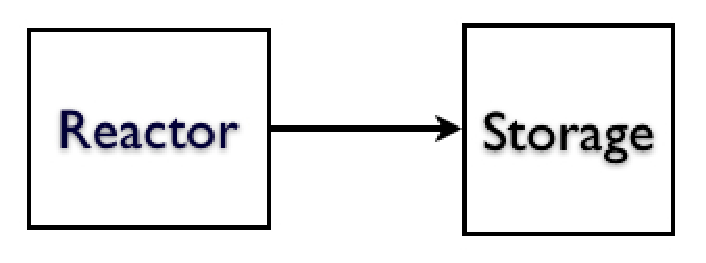
\includegraphics[width=0.4\textwidth]{R-S} 
\caption{Shematic Pathway\label{fig:R-S} }
\end{figure}
\begin{center}
\begin{minipage}{\textwidth}
\begin{lstlisting}
CLASSLogger *Logger = new CLASSLogger("CLASS_OUTPUT.log",1,2);  
EvolutionData* myFuel_EvolutionData = new EvolutionData(Logger, "/PATH/EvolData.dat");

Storage* MyStorage = new Storage(Logger);

Reactor *MyReactor = new Reactor(Logger, myFuel_EvolutionData, MyStorage, 0, 40*365.25*24.3600, 900E6, 100, 45, 1);	
\end{lstlisting}
\end{minipage}
\end{center}

\subsection{Reactor with fixed fuel, a Pool and a Storage}
\begin{figure}[h!]
\centering
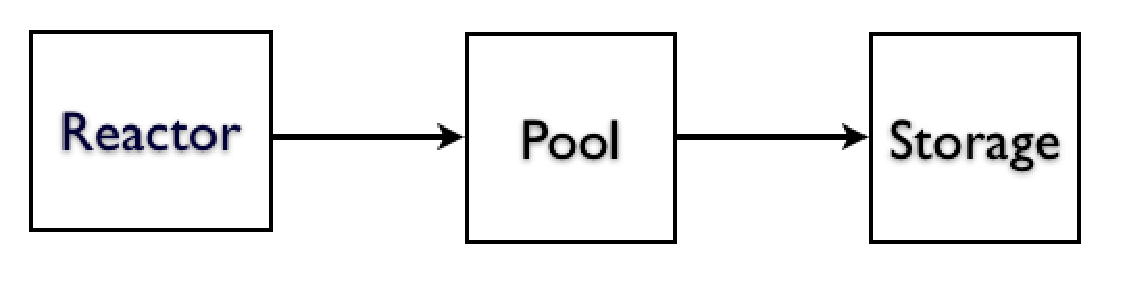
\includegraphics[width=0.6\textwidth]{R-P-S} 
\caption{Shematic Pathway\label{fig:R-P-S} }
\end{figure}

\begin{center}
\begin{minipage}{\textwidth}
\begin{lstlisting}
CLASSLogger *Logger = new CLASSLogger("CLASS_OUTPUT.log",1,2);  
EvolutionData* myFuel_EvolutionData = new EvolutionData(Logger, "/PATH/EvolData.dat");

Storage* MyStorage = new Storage(Logger);
Pool* MyPool = new Pool(Logger, MyStorage, 5*365.25*24*3600);

Reactor *MyReactor = new Reactor(Logger, myFuel_EvolutionData, MyPool, 0, 40*365.25*24.3600, 900E6, 100, 45, 1);	
\end{lstlisting}
\end{minipage}
\end{center}

\subsection{Reactor with fixed fuel, two SeprationPlant, a Pool and four Storage}
\begin{figure}[h!]
\centering
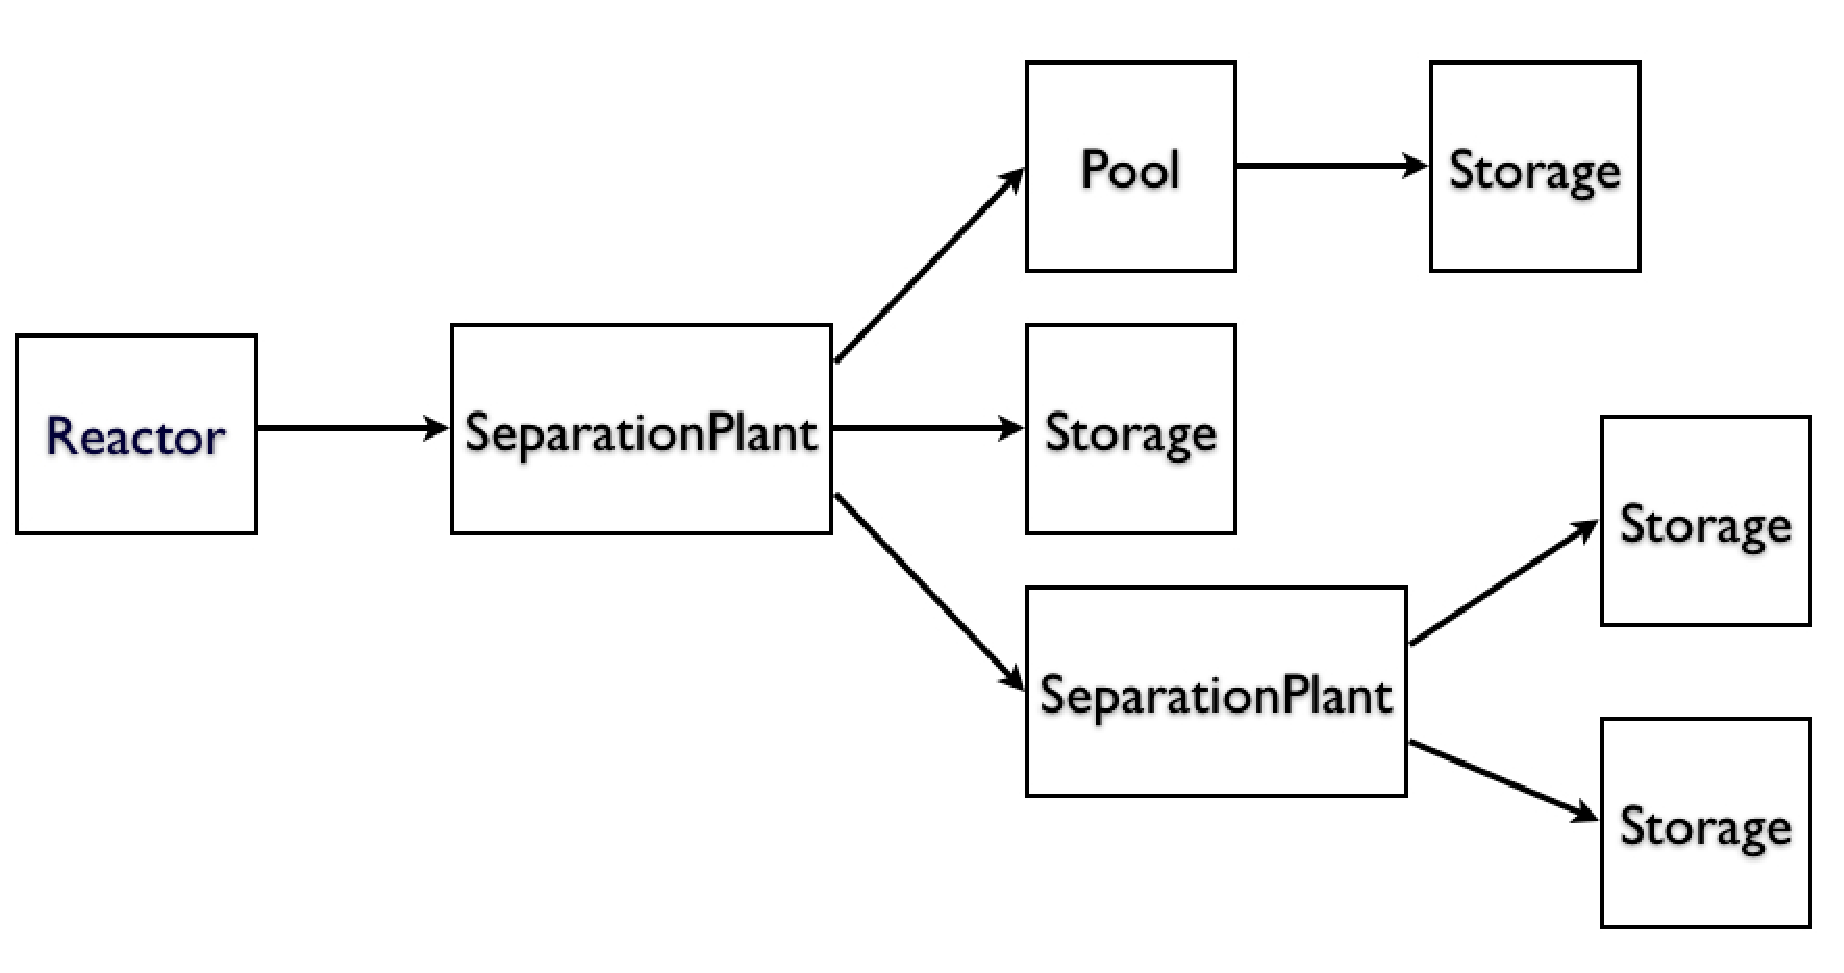
\includegraphics[width=1\textwidth]{R-SP-P_S-S-SP_S_S} 
\caption{Shematic Pathway\label{fig:R-SP-P_S-S-SP_S_S} }
\end{figure}
\begin{center}
\begin{minipage}{\textwidth}
\begin{lstlisting}
CLASSLogger *Logger = new CLASSLogger("CLASS_OUTPUT.log",1,2);  
EvolutionData* myFuel_EvolutionData = new EvolutionData(Logger, "/PATH/EvolData.dat");

Storage* MyStorage1 = new Storage(Logger);
Storage* MyStorage2 = new Storage(Logger);
Storage* MyStorage3 = new Storage(Logger);
Storage* MyStorage4 = new Storage(Logger);

Pool* MyPool1 = new Pool(Logger, MyStorage1, 5*365.25*24*3600);

// SeparationPlant separate U5 from U8 which goes in Storage 3 and 4.
SeparationPlan* MySeparation1 = new SeparationPlant(Logger);
IsotopicVector IV_U8;
IV_U8.Add(92, 238, 0, 1);
MySeparationPlant1->SetBackEndDestination(MyStorage3, IV_U8, 0);
					
IsotopicVector IV_U5;
IV_U5 += 1*ZAI(92, 235, 0);
MySeparationPlant1->SetBackEndDestination(MyStorage4, IV_U5, 0);
					

// SeparationPlant separate Am Pu and U which goes respectively in myPool1, myStorage2 and mySeparationPlan1.
SeparationPlan* MySeparation2 = new SeparationPlant(Logger);
IsotopicVector IV_MA;
IV_MA.Add(95, 242, 1, 1.);
MySeparationPlant2->SetBackEndDestination(MyPool1, IV_MA, 0);

IsotopicVector IV_Pu;
IV_Pu.Add(94, 239, 0, 0.8);
MySeparationPlant2->SetBackEndDestination(MyStorage2, IV_Pu, 0);
					
IsotopicVector IV_U;
IV_U.Add(92, 238, 0, 0.5);
IV_U.Add(92, 235, 0, 0.5);
MySeparationPlant2->SetBackEndDestination(MySeparationPlant1, IV_U, 0);

Reactor *MyReactor = new Reactor(Logger, myFuel_EvolutionData, MySeparation2, 0, 40*365.25*24.3600, 900E6, 100, 45, 1);	

\end{lstlisting}
\end{minipage}
\end{center}


\subsection{Reactor, a FabricationPlant, a Pool and a Storage}


\begin{center}
\begin{minipage}{\textwidth}
\begin{lstlisting}
CLASSLogger *Logger = new CLASSLogger("CLASS_OU TPUT.log",1,2);  

IM_RK4 *IMRK4 = new IM_RK4(Logger);
EQM_LIN_PWR_MOX* EQMLINPWRMOX = new EQM_LIN_PWR_MOX(Logger, "/PATH/EQ_Lin.dat");
EQM_QUAD_PWR_MOX* EQMQUADPWRMOX = new EQM_QUAD_PWR_MOX(Logger, "/PATH/DBParam.dat");
PhysicsModels* myFuel_PhysicsModel = new PhysicsModels(XSMOX, EQMQUADPWRMOX, IMRK4);

Storage* MyStorage = new Storage(Logger);
Pool* MyPool = new Pool(Logger, MyStorage, 5*365.25*24*3600);

FabricationPlant* myFabrication = new FabricationPlant(Logger, MyStorage, 2*365.25*24*3600);

Reactor *MyReactor = new Reactor(Logger, myFuel_PhysicsModel, myFabrication, MyPool, 0, 40*365.25*24.3600, 900E6, 100, 45, 1);	
\end{lstlisting}
\end{minipage}
\end{center}
\begin{figure}[h!]
\centering
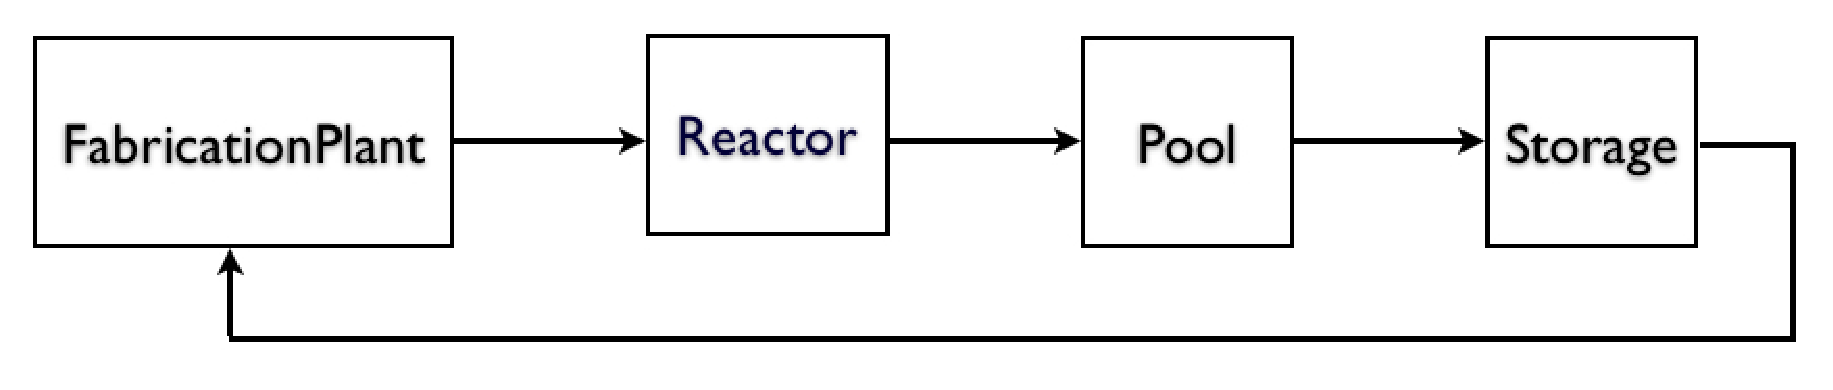
\includegraphics[width=0.9\textwidth]{FP_R_P_S} 
\caption{Shematic Pathway\label{fig:FP_R_P_S} }
\end{figure}

\chapter{Other objects}
\section{ZAI\label{sec:ZAI}}
The ZAi object represents a nucleus, from its charge number, mass number and isomeric state.\\
The object save  the charge number Z, the mass number A and the isomeric state I  of a nucleus : I=0 for ground state , I=1 for the first isomeric state ...\\
To declare a ZAI object proceed as follow :
\begin{center}
\begin{minipage}{\textwidth}
\begin{lstlisting}
ZAI U238 = ZAI(92, 238, 0);
\end{lstlisting}
\end{minipage}
\end{center}
This class includes the mains logical comparators (\emph{e.g} ==, >, !=). Fill free to read the doxygen for more details on the methods associated to this class. (\emph{e.g} A(), Z(), I(), N()...) \cite{doxygen}.
%\vspace{4cm}

\section{IsotopicVector\label{sec:IsotopicVector}}
\subsection{Generality}
The IsotopicVector object is a collection of ZAI, for each ZAI a number of nuclei is associated (IsotopicVector is a c++ map of ZAI and double, which corresponds to a sorted array of ZAI and its quantity).\\
Two pincipales operation have been defined on IsotopicVector. 
The following illustrates the possible operation allowed for IsotopicVectors :
\paragraph{Definiton \& Addition of nuclei}
\begin{center}
\begin{minipage}{\textwidth}
\begin{lstlisting}
IsotopicVector IV_1;
IsotopicVector IV_2;

IV_1 += 23 * ZAI(92, 238, 0); // Add 23 nucleus of uranium 238 to ZAI_1
IV_1 += 52 * ZAI(92, 235, 0); // Add 52 nucleus of uranium 235 to ZAI_1
\end{lstlisting}
\end{minipage}
\end{center}
\paragraph{Multiplication}
\begin{center}
\begin{minipage}{\textwidth}
\begin{lstlisting}
IV_1 *= 100; // Multiply all the nuclei quantities by 100 -> resulting : 2300 uranium 238 and 5200 uranium 235

IV_2 = IV_1 * 10; // IV_2 will be equal to 10 IV_1 
\end{lstlisting}
\end{minipage}
\end{center}
\paragraph{Sum}
\begin{center}
\begin{minipage}{\textwidth}
\begin{lstlisting}
IsotopicVector IV_sum = IV_1 + IV2; // IV_sum will be equal to 11 IV_1
\end{lstlisting}
\end{minipage}
\end{center}

Some additional operations have been also implemented, such as subtraction. It works as the sum, but if the result of the subtraction is negative for some nuclei, those nuclei are set to zero and the difference is added to the, so called, \textit{fIsotopicQuantityNeeded}. If so, a WARNING will be written on the terminal.\\
@@ Link WARNING \\
\textbf{To insure the quality and the reliability of the simulation, the fIsotopicQuantityNeeded MUST remain empty.}


\subsection{Print method}
You can use the Print() method to write the composition of an IsotopicVector.
When printing the IsotopicVector composition present nuclei, as well as the \textit{needed} one, are written with their corresponding quantity (unit: nucleus number).\\


\subsection{GetTotalMass}
Return the mass of the IsotopicVector in tons using :
\begin{center}
\begin{minipage}{\textwidth}
\begin{lstlisting}
double TotalMass = IV.GetTotalMass();
\end{lstlisting}
\end{minipage}
\end{center}


\subsection{Multiplication between IsotopicVector}
The result of this operation is an IsotopicVector, where each nucleus quantity is the product of the corresponding nucleus quantity of the two IsotopicVector.\\
In other words :\\
If a nucleus A is present in both IsotopicVector, with respective quantity $\alpha$ and $\beta$, the resulting IsotopicVector will contain $\alpha\times\beta$ nucleus A. If the nucleus A is not present in both IsotopicVector, the resulting IsotopicVector will not contain the nucleus A.\\

\textit{By exemple, this method can be used to apply separation efficiency: one IsotopicVector containing real material and the other one containing separation efficiency of each nucleus.}

\section{EvolutionData}\label{sec:EvolutionData}
An EvolutionData aims to describe the evolution of an \hyperref[sec:IsotopicVector]{IsotopicVector} through a physical process (decay or irradiation). The Decay case is fully described in section~\ref{sec:DecayDB}.\\

In case of irradiation, it may also contains the evolution of the one group cross section, the evolution of the neutron flux and the keff and are not mandatory. Note that neutron flux and keff are not used in CLASS. The EvolutionData MUST contain the power and can contain the heavy metal mass, the fuel type, reactor type and the cycle time.\\
These EvolutionData can be loaded into CLASS from a formatted ASCII file see section~\ref{sec:EDformat} as follow :

\begin{center}
\begin{minipage}{\textwidth}
\begin{lstlisting}
CLASSLogger *Logger = new CLASSLogger("CLASS_OUTPUT.log",1,2);  
 
EvolutionData*  MyEvolutionData = new EvolutionData(Logger, "/PATH/Data.dat");
\end{lstlisting}
\end{minipage}
\end{center}


\subsection{EvolutionData ASCII format}\label{sec:EDformat}
The formatted ASCII file describing the EvolutionData is formatted as follow:
\begin{center}
\begin{minipage}{\textwidth}
\begin{lstlisting}[label=lst:DatFormat,caption=Evolution Data format]
time "0 t2 t3 ..."						// in seconds
keff "k1 k2 k3 ..."					// not mandatory entry
flux "phi1 phi2 phi3 ..." 			//(neutron/(second.cm2))not mandatory entry
Inv "Z A I inv1 inv2 inv 3 ..."		//in atoms
...
XSFis "Z A I xsfis1 xsfis2 xsfis3 ..."//in barns
... 
XSCap "Z A I xscap1 xscap2 xscap3 ..."
...
XSn2n "Z A I xsn2n1 xsnsn2 xsn2n3 ..."
...
\end{lstlisting}
\end{minipage}
\end{center}

The meaning of each keyword is listed in table~\ref{tab:meanKeyWord}.

\begin{table}[H]
\begin{center}
\caption{.dat Key words meaning}
\label{tab:meanKeyWord}
\begin{tabular}{|c|c|}
\hline
Key words & Meaning \\
\hline
Inv & Inventory \\
\hline
XSFis &   fission cross section \\
XSCap & $(n,\gamma)$ cross section\\
XSn2n  &  $(n,2n)$ cross section \\
\hline
\hline
Value & meaning \\
\hline
Z & Charge number\\
A & Mass number\\
I & State (fundamental=0, $1^{st}$ excited =1, ...) \\
\hline
\end{tabular}
\end{center}

\end{table}

Each EvolutionName.dat files comes with a EvolutionName.info file, which describes the reactor, it is formatted like this :

\begin{center}
\begin{minipage}{\textwidth}
\begin{lstlisting}
Reactor "ReactorName"		//What ever string without space
Fueltype "FuelName"			//What ever string without space
CycleTime "t"						//The final time simulated (@@BaM)
ConstantPower "P"				//Simulated power (in W)
\end{lstlisting}
\end{minipage}
\end{center}


\subsection{DecayDataBank}\label{sec:DecayDB}
The radioactive decay is handled by a DecayDataBank. The DecayDataBank contains an EvolutionData for each nucleus of the nuclei chart. 
Each EvolutionData describes the evolution of the nucleus and all its daughters as a function of the time. The depletion of an isotopic vector corresponds to the sum of all its nucleus depletion contribution.\\

In other words, in CLASS, for each nucleus of the chart, a depletion calculation has been performed and compiled in a DecayDataBank.\\
The determination  of an \hyperref[sec:IsotopicVector]{IsotopicVector} depletion is performed as follow :\\
First, one determines the depletion of each nucleus of the \hyperref[sec:IsotopicVector]{IsotopicVector} following the DecayDataBank, then sums all those contributions.

DecayDataBank can be defined as follow :

\begin{center}
\begin{minipage}{\textwidth}
\begin{lstlisting}
CLASSLogger *Logger = new CLASSLogger("CLASS_OUTPUT.log",1,2);

DecayDataBank* DecayDB = new DecayDataBank(Logger, "/PATH/Decay.idx");
\end{lstlisting}
\end{minipage}
\end{center}
In the previous example a DecayDataBank has been defined using the file Decay.idx file. This file lists all the path to EvolutionDatas (each one corresponding to the depletion of one nucleus). The format of the .idx file is the following :

\begin{center}
\begin{minipage}{\textwidth}
\begin{lstlisting}
Z1 A1 I1 PATH/ZAI1.dat
...
Zn An In PATH/ZAIn.dat
\end{lstlisting}
\end{minipage}
\end{center}
A DecayDataBank can be find in \$PATH\_TO\_CLASS/Data/@@@.


\section{Log management : CLASSLogger}\label{sec:CLASSLogger}
In CLASS, all messages are handled by the CLASSLogger object. There are 4 verbose levels, see table~\ref{tab:verblevel}.

\begin{table}[H]
\begin{center}
\caption{Verbose levels}
\label{tab:verblevel}
\begin{tabular}{|c|c|l|}
\hline
level \# & meaning & informations\\
\hline
0 & ERROR & This is the default. \textit{It makes the code to stop}\\
\hline
1 & WARNING & LVL 0 + something may go wrong but the code continue running\\
\hline
2 & INFO &  LVL 1 + simple informations about ongoing process \\
\hline
3 & DEBUG & LVL 2 + each method begin and end \\
\hline
\end{tabular}
\end{center}
\end{table}

There are two outputs for these messages : the standard output (terminal) and a logfile. For each output a verbose level can be assigned as follow :
\begin{center}
\begin{minipage}{\textwidth}
\begin{lstlisting}
CLASSLogger *Logger = new CLASSLogger("CLASS_OUTPUT.log",1,2);  
\end{lstlisting}
\end{minipage}
\end{center}
In the preceding example, verbose level 1 (WARNING) has been set for the terminal output and level 2 (INFO) for the second output which is the logfile named CLASS\_OUTPUT.log. 

\chapter{Scenario/Park}
The Scenario object aims to describe the full scenario, regrouping all facilities inside a full park or fleet.

\section{Fill the scenario}
Each facilities to be able to evolve during a dynamic fuel cycle calculation need to be added inside the scenario. To do so five adding method have been implemented :

\begin{center}
\begin{minipage}{\textwidth}
\begin{lstlisting}
CLASSLogger *Logger = new CLASSLogger("CLASS_OUTPUT.log",1,2);
Scenario *gCLASS=new Scenario(Logger, 1977*year);

gCLASS->AddPool(myPool);					
gCLASS->AddReactor(myReactor);				
gCLASS->AddStorage(myStorage);				
gCLASS->AddFabricationPlant(myFabricationplant);
gCLASS->AddSeparationPlant(mySeparationplant);
//or
gCLASS->Add(myPool);
gCLASS->Add(myReactor);				
gCLASS->Add(myStorage);				
gCLASS->Add(myFabricationplant);
gCLASS->Add(mySeparationplant);
\end{lstlisting}
\end{minipage}
\end{center}

Furthermore, one need to add a DecayDataBase to the Scenario, using :

\begin{center}
\begin{minipage}{\textwidth}
\begin{lstlisting}
DecayDataBank* DecayDB = new DecayDataBank(Logger, "/PATH/Decay.idx");

gCLASS->SetDecayDataBase(DecayDB);
\end{lstlisting}
\end{minipage}
\end{center}


\section{OutPut}
\subsection{General Output}
In addition to all facilies added to the Scenario, the output contain also other general information.

\begin{table}[H]
\begin{center}
\caption{General Information in CLASS Output}
\label{tab:verblevel}
\begin{tabular}{|c|c|l|}
\hline
Output Name			&	Unit 				&	description\\
\hline
AbsoluteTime			&	Number [Second]			&	Time at the step\\	
\hline
\multirow{2}{*}{ParcPower}	&	\multirow{2}{*}{Number [Watt]}	&	Effective thermal power of the Scenario \\
				&					&	\textit{only working reactor are taked into account}\\	
\hline
WASTE				&	IsotopicVector			&	Waste produced by the scenario\\	
\hline
STOCK				&	IsotopicVector			&	All the material in all the Storage\\
\hline
OUTINCOME			&	IsotopicVector			&	All material taking from outside the Scenario\\
\hline
COOLING				&	IsotopicVector			&	All the material present in all the Pool\\
\hline
FUELFABRICATION			&	IsotopicVector			&	All the material present in all the FabricationPlant\\
\hline
REACTOR				&	IsotopicVector			&	All the material present in all the Reactor\\
\hline
\multirow{2}{*}{INCYLE}		&	\multirow{2}{*}{IsotopicVector}	&	All the material in the cycle\\
				&					&	\textit{Reactor + Pool + Fabrication + Storage}\\
\hline
\multirow{2}{*}{TOTAL}		&	\multirow{2}{*}{IsotopicVector}	&	All the material in the Scenario\\ 
				&					&	\textit{Reactor + Pool + Fabrication + Storage + Waste}\\	
\hline
\end{tabular}
\end{center}
\end{table}

\subsection{Output names}
The CLASS output is done in ROOT format, each element of the Scenario is added to a ROOT TTree, filled at each time step.
By default the output file name is "CLASS\_Default.root" and the ROOT TTree name is "Data". It is possible to change those names using :
\begin{center}
\begin{minipage}{\textwidth}
\begin{lstlisting}
gCLASS->SetOutputFileName("MyFileName.root");	
gCLASS->SetOutputTreeName("MyTTreeName");
\end{lstlisting}
\end{minipage}
\end{center}

\subsection{Output Frequency}
By default the output is done every years of simulation. To have more frequent (or less) output use :
\begin{center}
\begin{minipage}{\textwidth}
\begin{lstlisting}
gCLASS->SetTimeStep(365.25*24*3600/12); // monthly output	
\end{lstlisting}
\end{minipage}
\end{center}











%%%%%%%%%%%%%%%%%%%
%%%%%%
%% CHAPTER :		Physics MODEL
%%%%%%%%%%%%%%%%%%%%%%%%%
% !TEX root = USEGUIDE.tex

\part{Physics Models\label{sec:PhysicsModels}}
\chapter{Description and implementation}
A PhysicsModels is related to one or several reactors, it is a container of three models :
\begin{itemize}
\item Equivalence Model : Tells to the Fabrication Plant how to build the fuel.
\item XS Model : "Calculates" the mean  cross sections of this fuel and sends it to the Bateman Solver.
\item Irradiation Model : It is the Bateman Solver. User can choose between different numerical methods.
\end{itemize}

A PhysicsModels is called in the CLASS input like the following example :

\begin{center}
\begin{minipage}{\textwidth}
\textbf{Implementation in a .cxx :}
\begin{lstlisting}[label=lst:PIMP_HYMOD, caption=PhysicsModels]
...
#include "XS/XSM_MLP.hxx"
#include "Irradiation/IM_RK4.hxx"
#include "Equivalence/EQM_MLP_PWR_MOX.hxx"
int main()
{
	....

	EQM_MLP_MOX* Equivalence 	= new EQM_MLP_MOX( "PathToTMVAWeightFile/TMVAWeightFile.xml" );
	XSM_MLP* XS = new XSM_MLP( gCLASS->GetLog(),"PathToTMVAWeighstFolder" , OneMLPPerTimeStep );
	IM_RK4* Solver = new IM_RK4( gCLASS->GetLog() );
	PhysicsModels* PHYMOD = new PhysicsModels( XS , Equivalence , Solver );
	
	...
	Reactor *PWR_MOX = new Reactor(log, PHYMOD, fabricationplant, Pool, creationtime, lifetime, cycletime, HMMass, BurnUp);
	...
}			
\end{lstlisting}
\end{minipage}
\end{center}

In this latter example a PhysicsModels called "PHYMOD" is defined, it contains the bateman solver "Solver" which is the Runge Kutta ($4^{th}$ order) method. The mean cross sections predictor, "XS",  used is  based on a Multi Layer Perceptron. The Equivalence Model "Equivalence" is the one used for PWR MOX fuels. The arguments of the 3 objects constructor are explained in its corresponding sections.

All the existing models are defined in the following sections, furthermore, the way to build a new model is presented.




%%%%%%%%%%%%%%%%%%%%%%%%%
%%		EQUIVALENCE MODEL
%%%%%%%%%%%%%%%%%%%%%%%%%
\chapter{Equivalence Model}\label{sec:EquivalenceModel}
The aim of an equivalence model is to predict the content of fissile element needed in a fuel to reach a given burn-up or to satisfied criticality conditions.
\section{Available Equivalence Models}
The CLASS package contains, at the moment, 4 different equivalence models where three are related to the building of fuels for a PWR-MOX and one to the building of  PWR-UOX fuels :
\subsection{PWR-MOX models :}
The following models returns the molar fraction $\%_{Pu}$ of plutonium needed to reach a given burn-up according to the plutonium isotopic composition available in stocks.



\subsubsection{Linear BU model : EQM\_LIN\_MOX } 
It was initially applied for MOX fuel, but because of the lack of precision, this model could be deprecated (at least in the PWR MOX case). It remain in the CLASS packages only because it was present historically.\\
 Nevertheless it could be use as an example for similar model for other fuel. This model suppose it is possible to describe the maximal burn-up accessible for a set fuel using its initial composition using a simple linear modelisation (equation~\ref{eq:EQM_LIN}):\\ 
\begin{equation}\label{eq:EQM_LIN}
BU_{max} = \alpha_{0} +   \sum_{i}^{N} \alpha_{i} \cdot n_{i},
\end{equation}
where $BU_{max}$ represent the maximal accessible burn-up for the fuel, $n_{i}$ the isotopic fraction of the isotope $i$, $N$ the number of isotope present in the fuel, and the $\alpha_{i}$ the parameter of the model. 
The main difficulty concerning this model, is the determination of the $\alpha_{i}$: to be correct the $\alpha_{i}$ should be fitted on a set of evolution data which are not constrain to reach an unique burn-up, but a large burn-up region. One can see the problem guessing it is possible to build a set a fuel evolution reaching exactly a unique burn-up (45 GWd/t by example), the $\chi^{2}$ minimization of the $\alpha_i$ will end up with $\alpha_{0} = 45$ and all the other at zero. That why, when using a linear burn-up description model, one should test the validity of the model, on many random compositions by example... 

\subsubsection{Quadratic Model : EQM\_QUAD\_MOX}
The $\%_{Pu}$ is calculated according a quadratic model. See equation~\ref{eq:EQM_QUAD_MOX}.
\begin{equation}\label{eq:EQM_QUAD_MOX}
\%_{Pu} = \alpha_{0} +   \sum_{i\in Pu}^{N} \left(\alpha_{i} \cdot n_{i}\ + \sum_{j\leq i} \alpha_{ij} \cdot n_{i}\cdot n_{j}\right),
\end{equation}
where $n_{i}$ is the molar proportion (in $\%mol.$) of isotope $i$ \footnote{from $^{238}Pu$ to $^{242}Pu$} in the fresh plutonium vector.  $\alpha_{ij}$, $\alpha_{i}$ and $\alpha_{0}$  are the weights resulting from a minimization procedure and are related to one targeted burn-up and one fuel management. Furthermore, $^{241}Am$ from $^{241}Pu$ decay is not one of the considered component of the model ($n_{i}$), instead the model considers a fixed time since plutonium separation. For instance the $\alpha$ given in file \$CLASS\_PATH/DATA\_BASES/PWR/MOX/EQModel/@@BAM
are representative of a PWR-MOX with a maximal burn-up of $45GWd/tHM$, a fuel management of 3 batches, and a time between separation and irradiation of 2 years.

The file containing the weights is formatted as follow :

\begin{center}
\begin{minipage}{\textwidth}
\begin{lstlisting}
PARAM "238Pu 238Pu*238Pu 238Pu*239Pu 238Pu*240Pu 238Pu*241Pu 238Pu*242Pu 239Pu 239Pu*239Pu 239Pu*240Pu 239Pu*241Pu 239Pu*242Pu 240Pu 240Pu*240Pu 240Pu*241Pu 240Pu*242Pu 241Pu 241Pu*241Pu 241Pu*242Pu 242Pu 242Pu*242Pu 1"
\end{lstlisting}
\end{minipage}
\end{center}

Where 238Pu stands for $\alpha_{^{238}Pu}$ and it is the first order weight  related to the  molar proportion of $^{238}Pu$ and $1$ is $\alpha_{0}$. The weights are in units of $\%mol. \cdot \%mol.^{-1}$ for $\alpha_{i}$ in units of  $\%mol. \cdot \%mol.^{-2}$ for  $\alpha_{ij}$ and in units of $\%mol.$ for $\alpha_{0}$. The Keyword "PARAM" has to be present in the file before the $\alpha$ values. For more informations about this model and the generation of the coefficients please refer to reference [@@PAPIER BAM].
\\  
\\

\begin{center}
\begin{minipage}{\textwidth}
\textbf{Implementation in a .cxx }
\begin{lstlisting}[label=lst:IMP_EQMQUAD,caption=Equivalence Model EQM\_QUAD\_MOX ]
...
#include "Equivalence/EQM_QUAD_PWR_MOX.hxx"
...
int main()
{
...
EQM_QUAD_PWR_MOX* Equivalence = new	EQM_QUAD_PWR_MOX( LogObject, AlphasFile );
// or
// EQM_QUAD_PWR_MOX* Equivalence = new	EQM_QUAD_PWR_MOX( AlphasFile );
...
}
\end{lstlisting}
\end{minipage}
\end{center}

With LogObject a \hyperref[sec:CLASSLogger]{CLASSLogger} object (see section~\ref{sec:CLASSLogger}) and AlphasFile a string which is the complete path to the file containing the weights (the $\alpha$ parameters)
\\
\\

\begin{center}
\begin{minipage}{\textwidth}
\textbf{Available weight file (.dat) : }
\begin{itemize}
\item \textbf{@@@ BAM}
\item \textbf{@@@ BAM}
\item ...
\end{itemize}
\end{minipage}
\end{center}

\subsubsection{Neural network model : EQM\_MLP\_MOX}\label{sec:EQMMOX}
This equivalence model  is based on a Multi Layer Perceptron (MLP) and  predict the amount of plutonium needed to reach \textbf{any burn-up}. The MLP inputs are the isotopic compositions of the plutonium (\textbf{including $^{241}Am$}), the enrichment of depleted uranium, and the targeted burn-up. The output is the plutonium content needed to reach the burn-up. This method uses the neural networks of the root module TMVA (@@@  Ref TMVA). To executes this model, TMVA is run in CLASS and need a .xml file. This file contains the neural network architecture and the weights resulting from the training procedure.
\\
\\
\begin{center}
\begin{minipage}{\textwidth}
\textbf{Implementation in a .cxx : }
\begin{lstlisting}[label=lst:IMP_EQMMLP,caption=Equivalence Model EQM\_MLP\_PWR\_MOX ]
...
#include "Equivalence/EQM_MLP_PWR_MOX.hxx"
...
int main()
{
...
EQM_MLP_PWR_MOX* Equivalence = new	EQM_MLP_PWR_MOX( LogObject, TMVAWeightPath );
// or
// EQM_MLP_PWR_MOX.* Equivalence = new	EQM_MLP_PWR_MOX( TMVAWeightPath );
...
\end{lstlisting}
\end{minipage}
\end{center}

With LogObject a \hyperref[sec:CLASSLogger]{CLASSLogger} object (see section~\ref{sec:CLASSLogger}) and TMVAWeightPath a string containing the path to the .xml file. 


In order to make his own .xml file one need to have a training data containing the fresh fuel composition and the achievable burn-up of many examples. The fuel composition is characterized by the mean of :
\begin{itemize}
\item The plutonium composition (\emph{i.e :} \%mol. of $^{238}Pu$, $^{239}Pu$, $^{240}Pu$, $^{241}Pu$, $^{242}Pu$, and $^{241}Am$)
\item The plutonium content (\emph{i.e :}  $\frac{Pu}{Pu+U}$)
\item The $^{235}U$ content in the depleted uranium.
\end{itemize}

The file \$CLASS\_PATH/DATA\_BASES/PWR/MOX/EQModel/EQM\_MLP\_PWR\_MOX\_3batch.xml has been generated from the file \$CLASS\_PATH/Utils/Equivalence/PWR\_MOX\_MLP/Train\_MLP.cxx 
To train a new MLP from your own training sample proceed as follow : 
\begin{center}
\begin{minipage}{\textwidth} 
\begin{lstlisting}[style=terminal]
cd $CLASS_PATH/Utils/Equivalence/PWR_MOX_MLP
g++ -o Train_MLP `root-config --cflags` Train_MLP.cxx `root-config --glibs` -lTMVA -I$ROOTSYS/tmva/test/
Train_MLP YourTrainingData.root
\end{lstlisting}
\end{minipage}
\end{center}


Where YourTrainingData.root is a root file containing a TTree filled with fuel compositions and corresponding burn-ups. The .xml file will be generated in a folder named weight. The results of the testing procedure of the MLP are in a file named TMVA\_MOX\_Equivalence.root but will be presented to you graphically as soon as the training and the testing procedure are finished.

To make your YourTrainingData.root file you have to fill a TTree with your data. To do so, create a .cxx file and copy past this :

\begin{center}
\begin{minipage}{\textwidth}
\begin{lstlisting}
	TFile*   fOutFile = new TFile("YourTrainingData.root","RECREATE"); //create the .root file
	TTree*   fOutT = new TTree("Data", "Data");//create the TTree
/**********************INITIALISATIONNN********************/
//WARNING : keep the same variable names :
	double U5_enrichment  = 0;
	double Pu8 				 = 0;
	double Pu9 				 = 0;
	double Pu10 			 = 0;
	double Pu11				 = 0;
	double Pu12 	     = 0;
	double Am1 	    	 = 0;
	double BU 				 = 0;   //BU means Burn-Up
	double teneur 		  = 0;	//French for content (here Pu content)
/**********************BRANCHING**************************/
	fOutT->Branch(	"U5_enrichment"	,&U5_enrichment	,"U5_enrichment/D"	);
	fOutT->Branch(	"Pu8"			,&Pu8			,"Pu8/D"			);
	fOutT->Branch(	"Pu9"			,&Pu9			,"Pu9/D"			);
	fOutT->Branch(	"Pu10"		,&Pu10		,"Pu10/D"			);
	fOutT->Branch(	"Pu11"		,&Pu11		,"Pu11/D"			);
	fOutT->Branch(	"Pu12"		,&Pu12		,"Pu12/D"			);
	fOutT->Branch(	"Am1"			,&Am1			,"Am1/D"			);
	fOutT->Branch(	"BU"			,&BU			,"BU/D"				);
	fOutT->Branch(	"teneur"	,&teneur	,"teneur/D"			);
/**********************FILLING******************************/
//	int Nex=NumberOfDifferentExample;
	for(int ex=0;ex<Nex;ex++)
	{ /*******Fresh Fuel Composition***********/
		U5_enrichment 	=  fU5_enrichment[ex]; 
		Pu8  	  		=  fPu8[ex];
		Pu9  	  		=  fPu9[ex];
		Pu10 	  		=  fPu10[ex];
		Pu11 	  		=  fPu11[ex];
		Pu12 	  		=  fPu12[ex];
		Am1 	  		=  fAm1[ex];
		teneur 	  	=  fteneur[ex];
		/*****Corresponding maximal Burn-up*******/
		BU   	  		=  BurnUps[ex]; 
		/****Fill the tree with this fuel composition and this burnup****/
		fOutT->Fill();
	}
	fOutFile->Write();
	delete fOutT;
	fOutFile-> Close();
	delete fOutFile;
}
\end{lstlisting}
\end{minipage}
\end{center}

Then, build the arrays fU5\_enrichment, fPu8 ... with your data, compile and execute.
For more informations about this model please refer to [@@Papier BaL].\\
\textbf{Available weight file (.xml) : }
\begin{itemize}
\item \textbf{\$CLASS\_PATH/DATA\_BASES/PWR/MOX/EQModel/EQM\_MLP\_PWR\_MOX\_3batch.xml} : Generated with 5000 MURE evolutions with different fuel composition, using a full mirrored assembly calculation with JEFF3.1.1 cross section and fission yield data bases. Valid for mono-recycling of plutonium and a fuel management of 3 batches. More details about the generation of this .xml file can be found in reference[@@@BaL paper].
\end{itemize}


\subsection{PWR-UOX model :}

\subsubsection{Linear Model: EQM\_LIN\_UOX}
@@@BAM

\section{How to build an Equivalence Model}
The strength of CLASS is to allow the user to build his own Physics models, this section explains how to build a new equivalence model and to incorporate it into CLASS.

First you have to create the file EQM\_NAME.cxx and EQM\_NAME.hxx, where NAME is a name you choose. 
Then open with a text editor the .hxx and copy past the following replacing NAME by the name you want.

\begin{center}
\begin{minipage}{\textwidth}
\begin{lstlisting}[label=lst:HXX_EQM,caption=EQM\_NAME.hxx ]
#ifndef _EQM_NAME_HXX
#define _EQM_NAME_HXX
#include "EquivalenceModel.hxx"
using namespace std;
//---------------------------------------------------------//
/*!
 Define a EQM_NAME
  Explain briefly what is it.
  @author YourName
  @version 3.0
 */
//________________________________________________________________________
class EQM_NAME : public EquivalenceModel
{
	public :
	/*Constructor*/
	EQM_NAME(/*parameters*/ ); //!< Explain what is the parameters (if any) 

	/**This function IS the equivalence model **/	
	double GetFissileMolarFraction(IsotopicVector Fissil,IsotopicVector Fertil,double BurnUp); //!<Return the molar fraction of fissile element 

	private :
	/*Your private variables*/
};
#endif
\end{lstlisting} 
\end{minipage}
\end{center}

Open the .cxx file and copy past the following in it (replacing NAME by the same name you used in the .hxx).
 
\begin{center}
\begin{minipage}{\textwidth}
\begin{lstlisting}[label=lst:CXX_EQM,caption=EQM\_NAME.cxx ]
#include "EquivalenceModel.hxx"
#include "EQM_NAME.hxx"
#include "CLASSLogger.hxx"
/*Whatever include you need*/
//________________________________________________________________________
//		EQM_NAME
//
//	Brief description
//________________________________________________________________________
//Constructor(s)
EQM_NAME::EQM_NAME(/*parameters*/)
{
//.... Do whatever you want with your parameters
/*
	Fill the two isotopic vectors fFissileList and fFertileList 
	see explanation in the manual
*/
	//Fertile
	ZAI U8(92,238,0);
	ZAI U5(92,235,0);
	double U5_enrich= 0.0025;
	fFertileList = U5*U5_enrich + U8*(1-U5_enrich);

	//Fissile
	ZAI Pu8(94,238,0);
	ZAI Pu9(94,239,0);
	//...
	fFissileList = Pu8*1+Pu9*1+ /*...*/;
}
//_______________________________________________________________________
double EQM_NAME::GetFissileMolarFraction(IsotopicVector Fissil,IsotopicVector Fertil,double BurnUp)
{
//Code your Equivalence Model : This function has to return the molar fraction	of fissile in the fuel needed to reach the BurnUp(GWd/tHM) according to the composition of the Fissil and Fertil vectors 
}
\end{lstlisting} 
\end{minipage}
\end{center}

In the constructor (EQM\_NAME::EQM\_NAME) you have to fill two isotopic vectors named \textbf{fFissileList} and \textbf{fFertileList}. Don't declare these isotopic vector in the .hxx, there are already declared in the file src/EquivalenceModel.hxx. fFissileList is used by the FabricationPlant to do the chemical separation of the fissile element from the other present in stock. For instance, for the plutonium, add the ZAI $^{238}Pu$, $^{239}Pu$, $^{240}Pu$, $^{241}Pu$ and $^{242}Pu$. fFertile List is used by the FabricationPlant the same way fFissileList is used but you have to define a default \hyperref[sec:IsotopicVector]{IsotopicVector} to be used if you didn't provide a fertile stock to your FabricationPlant.  In the example given above the fertile is depleted uranium and  the proportion of each isotope is given ($^{234}U$ is unheeded). Now you have to build the function \textbf{GetFissileMolarFraction(IsotopicVector Fissil, IsotopicVector Fertil, double BurnUp)}. Its parameters are provided by the FabricationPlant and are :

\begin{itemize}
\item \hyperref[sec:IsotopicVector]{IsotopicVector} Fissile : it is the proportion of each nucleus you give in the fFissileList plus the proportion of the nuclei that appears during the fabrication time (time given in the FabricationPlant constructor, is default is 2 years)
\item \hyperref[sec:IsotopicVector]{IsotopicVector} Fertile :  it is the proportion of each nucleus you give in the fFertileList plus the proportion of the nuclei that appears during the fabrication time. If you didn't provide any fertile stock to your FabricationPlant then it's the default vector given in the EQM\_NAME constructor.
\item double BurnUp : The maximal average burn-up for your fuel to reach (in GWd/tHM).
\end{itemize}
Fill free to have a look at the models present in \$CLASS\_PATH/source/Model/Equivalence to get inspiration.

Now that your equivalence model is ready two choices are offered to you. You can compile the two files of your model with your CLASS input or you can add this model to the CLASS package. The second option will modify the CLASS software and we will be no longer able to troubleshoot your scenario. So use the second option only if you are a completely independent user !

\subsection{Compile your equivalence model with your CLASS executable :}
@@BAM

\subsection{Your equivalence model in the CLASS library :}
Move your  EQM\_NAME.hxx and  EQM\_NAME.cxx in \$CLASS\_PATH/source/Model/Equivalence/. Then open with your favourite text editor the file  \$CLASS\_PATH/source/src/Makefile, find "OBJMODEL" and add \$(EQM)/EQM\_NAME.o within the others \$(EQM) objects. Then re-compile CLASS, fix the compilation errors ;) and voil� your equivalence model is now available in the CLASS library.




%%%%%%%%%%%%%%%%%%%%%%%%%
%%		XS MODEL
%%%%%%%%%%%%%%%%%%%%%%%%%
\chapter{XS Model}
The aim of a mean cross section model (XSModel) is to predict the mean cross sections of a fuel built by an EquivalenceModel (EQM) (see section \ref{sec:EquivalenceModel}). The mean cross sections are required to compute fuel depletion in a reactor.

\section{Available XS Models}
There is, for the moment, 2 XSModel in CLASS : 
\subsection{Pre-calculated XS : XSM\_CLOSEST}\label{sec:CLOSEST}
This method looks, in a data base, for a fresh fuel with a composition \textbf{close} to the brandy new fuel built by the EquivalenceModel. Here, close means that the fresh fuel in the data base minimizes the distance $d$ (see equation~\ref{eq:distance}).
\begin{equation}\label{eq:distance}
d=\sqrt{\sum_{i} w_{i}\cdot(n_{i}^{DB} - n_{i}^{new} )^{2} },
\end{equation}
where $n_{i}^{DB}$ is the number of nuclei $i$ in one element of the data base and  $n_{i}^{new}$ the number of nuclei $i$ in the new fuel built by the EQM. $w_{i}$ is a weight associated to each isotopes, its value is 1 by default.
When the closest evolution in the database is found, the corresponding mean cross sections are extracted and used for the calculation of the depletion of the new fuel.
\\
\\
\begin{center}
\begin{minipage}{\textwidth}
\textbf{Implementation in a .cxx : }
\begin{lstlisting}[label=lst:IMP_EQMQUAD,caption=Cross section Model XSM\_CLOSEST ]
...
#include "XS/XSM_CLOSEST.hxx"
...
int main()
{
	XSM_CLOSEST* XSMOX = new XSM_CLOSEST( gCLASS->GetLog(), PathToIdxFile );
	//or
	//XSM_CLOSEST* XSMOX = new XSM_CLOSEST( PathToIdxFile );
}
\end{lstlisting}
\end{minipage}
\end{center}

With LogObject a \hyperref[sec:CLASSLogger]{CLASSLogger} object (see section~\ref{sec:CLASSLogger}) and PathToIdxFile  a string containing the path to the .idx file. The .idx file lists all the EvolutionData (see section~\ref{sec:EvolutionData}) of the data base. This file is formatted as follow :

\begin{center}
\begin{minipage}{\textwidth}
\begin{lstlisting}
TYPE "NameOfTheFuel(withoutspace)"
"PATH_TO_DATA_BASE/EvolutionName.dat"
"PATH_TO_DATA_BASE/OtherEvolutionName.dat"
....
\end{lstlisting}
\end{minipage}
\end{center}

Each EvolutionName.dat file contains a formatted fuel depletion calculation. the format of a EvolutionData ASCII file is detailed in section~\ref{sec:EDformat}.  The number of .dat files has an influence on the model accuracy. Furthermore, the initial composition of the different fuel depletion calculations has to be representative of the fresh fuel compositions encounter in a scenario. For more details on this method please refer to [ref @@@ BAM physor]. 


\textbf{Available .idx file  : }
\begin{itemize}
\item \textbf{@@@ BAM}
\item \textbf{@@@ BAM}
\item ...
\end{itemize}

\textbf{For MURE user only : } The program \$CLASS\_PATH/Utils/XS/CLOSEST/WriteDataBase converts a list of MURE evolutions to a list of .dat and .info files and creates the .idx file, type in terminal the following command for more details.

\begin{center}
\begin{minipage}{\textwidth}
\begin{lstlisting}[style=terminal]
\$CLASS\_PATH/Utils/XS/CLOSEST/WriteDataBase -h 
@@BAM
\end{lstlisting}
\end{minipage}
\end{center}

Users of others fuel depletion code (\emph{e.g} VESTA, ORIGEN, MONTEBURNS, SERPENT .... ) have to create their own program to generate these files.




\subsection{XS predictor : XSM\_MLP}
This method calculates the mean cross sections by the mean of a set of neural networks (MLP from TMVA module) . There is two configurations available :

\begin{itemize}
\item One MLP per nuclear reaction and per time step (this one is deprecated and not describe in this manual) .
\item	One MLP per nuclear reaction. the irradiation time is one of the MLP inputs.
\end{itemize}

\begin{center}
\begin{minipage}{\textwidth}
\textbf{Implementation in a .cxx : }
\begin{lstlisting}[label=lst:IMP_EQMQUAD,caption=Cross section Model XSM\_MLP ]
...
#include "XS/XSM_MLP.hxx"
...
int main()
{	...
	XSM_MLP* XSMOX = new XSM_MLP( ClassLog, PathToWeightFolder, InfoFileName, OneMLPPerTime );
//or
//XSM_MLP* XSMOX = new XSM_MLP(PathToWeightFolder, InfoFileName, OneMLPPerTime);
...
}
\end{lstlisting}
\end{minipage}
\end{center}
\textbf{PathToWeightFolder} (string) is the path to the folder containing the weight files (.xml files). \textbf{OneMLPPerTime} is a boolean setted to true if there is one MLP per reaction and per time step. \textbf{InfoFileName} (string) is the name of the file located in PathToWeightFolder which is informing on the reactor and on the inputs of the XS\_MLP model.
Format of InfoFileName is :
\begin{center}
\begin{minipage}{\textwidth}
\begin{lstlisting}[label=lst:informationfile,caption=Information file format]
ReactorType :"ReactorName"	//without space
FuelType :"FuelName" //without space
Heavy Metal (t) :"m"
Thermal Power (W) :"P"     //power corresponding to the heavy metal mass
Time (s) :"0 t2 t3 t4 ..." //Time when the cross section are updated
Z A I Name (input MLP) : //see explanations below
"z a i InputName"
"z2 a2 i2 InputName2"
"..."
\end{lstlisting}
\end{minipage}
\end{center}

The input of MLPs are the atomic proportion of each nuclei present in the fresh fuel (plus time if OneMLPPerTime=false). The InfoFile has to indicates the variable names (nuclei name) you used for the \textcolor{blue}{\textbf{training of your MLPs}}. For instance if the fresh fuel contains $^{238}Pu$ you will write in the InfoFile  :

\begin{center}
\begin{minipage}{\textwidth}
\begin{lstlisting}
...
Z A I Name (input MLP) :
94 238 0 Pu8//(if Pu8 is the variable name used for 238Pu proportion in fresh fuel in your training sample) 
...
\end{lstlisting}
\end{minipage}
\end{center}
\textbf{Available XSM\_MLP : }
\begin{itemize}
\item \$CLASS\_PATH/DATA\_BASES/PWR/MOX/XSModel/30Wg\_FullMOX :
The weight files and .nfo file contained in this folder are representative of a PWR MOX. With the MOX coming from PWR UO2 spent fuels. The specific power is 30W/g oxide. To perform this data base, MURE depletion calculations have been performed using a full MOX assembly with mirror boundaries. 
\end{itemize}

\textcolor{blue}{\large{\textbf{Training MLPs for cross sections prediction :}}}\\

\textbf{\underline{ Preparation of the training sample :} }\\
\\
Like for the equivalence model, first of all you have to create a training sample. This is one of the most important thing since the way of filling the hyperspace of the MLP inputs will influence the accuracy of your model. We suggest to used the Latin Hyper Cube method [@@@REFF] to generate many fresh fuel compositions, then, calculates with your favourite neutron transport code (MCNP, MORET, SERPENT ...) the mean cross sections of each fresh fuel for different irradiation time. Please refer to [REFFFBAL MLPXS] for more informations about the space filling and the validation of this cross sections predictor.
Once all your calculations are complete you have to convert them into the .dat format (see code frame~\ref{lst:DatFormat}).
Then type :

\begin{center}
\begin{minipage}{\textwidth}
\begin{lstlisting}[style=terminal]
cd $CLASS_PATH/Utils/XS/MLP/BuildInput
\end{lstlisting}
\end{minipage}
\end{center}

Open the file Gene.cxx, looks for @@Change and make the appropriate changes. Then type :

\begin{center}
\begin{minipage}{\textwidth}
\begin{lstlisting}[style=terminal]
g++ -o Gene Gene.cxx `root-config --cflags` `root-config --libs`
Gene PATH_To_dat_Folder/
\end{lstlisting}
\end{minipage}
\end{center}

Where  PATH\_To\_dat\_Folder/ is the path to the folder containing the .dat files. This program should have built two files :

\begin{itemize}
\item TrainingInput.root : This root file contains the fresh fuel inventories and the cross sections values of all the read .dat files. You can plot the data with the root command line tool if you wish. This file is the \textbf{Training and testing sample} that will be used for the TMVA training and testing procedure.
 
\item TrainingInput.cxx : This file contains, in a vector, the names of all the MLP outputs. The number of lines in this file is the number of MLP that will be train.
\end{itemize} 

\textbf{\underline{ Training and testing procedure : }}\\
\\
Once the two TrainingInput (.cxx and .root) are generated type :

\begin{center}
\begin{minipage}{\textwidth}
\begin{lstlisting}[style=terminal]
cd $CLASS_PATH/Utils/XS/MLP/Train
\end{lstlisting}
\end{minipage} 
\end{center}

 Look for @@Change in the file Train\_XS.cxx , and make the appropriate changes. Then type :

\begin{center}
\begin{minipage}{\textwidth}
\begin{lstlisting}[style=terminal]
 g++ -o Train_XS  `root-config --cflags` Train_XS.cxx `root-config --glibs` -lTMVA
\end{lstlisting}
\end{minipage} 
\end{center}

According the number of "events" in your .root file and the number of cross sections, the training time can be very very very long. You might want to decrease the number of events (this will probably deteriorate the model accuracy) : look for nTrain\_Regression in Train\_XS.cxx and change its value to your wanted number of events. And/Or you may want to use more than one processor or perhaps a supercomputer : This is completely doable since the program Train\_XS trains only one MLP (one cross section). Indeed the execution line is the following :

\begin{center}
\begin{minipage}{\textwidth}
\begin{lstlisting}[style=terminal]
Train_XS i
\end{lstlisting}
\end{minipage} 
\end{center}

where i is the index of the cross section in the vector created in TrainingInput.cxx. So feel free to create a script to run the training on a wanted number of processors. For instance let's say you have 40 cross sections and 4 processors, creates 4 files (make them executable) and in the first one type :

\begin{center}
\begin{minipage}{\textwidth}
\begin{lstlisting}
Train_XS 0
Train_XS 1
...
TrainXS 9
\end{lstlisting}
\end{minipage} 
\end{center}

continue in the second file, and so on. Then execute all of them. The architecture and weights of each MLP (.xml files) are stored in the folder weights. Rename this folder by the name of the reactor and fuel, then create in this folder the information file (see code frame~\ref{lst:informationfile}). And voil� your new XSM\_MLP is ready to be used.\\

After each training (using by default the half of the events) a testing procedure (using the other half) is performed. This latter consists on executing the trained MLP with input data from a known sample and compare the MLP result to the true value. These data and other informations about the training are stored in file \textbf{Training\_output\_i.root}, with i the index of the cross section. In order to see either the MLPs predictions are accurate or not, the root macro \$CLASS\_PATH/Utils/XS/MLP/Train/deviations.C plot the distribution of relative differences between model executions and the true values and a  Gaussian fit of it. Then, the mean and the standard deviation of the Gaussian fit are stored in file \textbf{XS\_accuracy.dat} (format : XSName mean std.dev.). Type the following to get, in file XS\_accuracy.dat, the mean and the standard deviation of all the MLPs (with N the number of cross sections (number of MLPs) ) :

\begin{center}
\begin{minipage}{\textwidth}
\begin{lstlisting}[style=terminal]
cd $CLASS\_PATH/Utils/XS/MLP/Train/
root
.L deviations.C
for(int i=0;i<N;i++) {stringstream ss;ss<<"Training_output_"<<i<<".root";deviations(ss.str().c_str(),0,kTRUE,kFALSE,kFALSE); }
\end{lstlisting}
\end{minipage} 
\end{center}
 
 The closest to 0 the mean is and the smaller standard deviation, the better.
 
 

\section{How to build an XS Model}
The strength of CLASS is to allow the user to build his own Physics models, this section explains how to build a new cross section model and to incorporate it into CLASS.
First you have to create the file XSM\_NAME.cxx and XSM\_NAME.hxx, where NAME is a name you choose. 
Then open with a text editor the .hxx and copy past the following replacing NAME by the name you want.

\begin{center}
\begin{minipage}{\textwidth}
\begin{lstlisting}[label=lst:HXX_XSM,caption=XSM\_NAME.hxx ]
#ifndef _XSM_NAME_HXX
#define _XSM_NAME_HXX
#include "XSModel.hxx"
// add include if needed
using namespace std;
//----------------------------------------------------------------------//
/*!
 Define a XSM_NAME
describe your model
 @authors YourName
 @version 1.0
 */
//________________________________________________________________________
class XSM_NAME : public XSModel
{
	public :
	
	XSM_NAME(/*parameters (if any)*/);

	~XSM_NAME();

 	EvolutionData GetCrossSections(IsotopicVector IV,double t=0);

	private :			
	//your private variables and methods
};
#endif
\end{lstlisting}
\end{minipage} 
\end{center}


Open the .cxx file and copy past the following in it (replacing NAME by the same name you used in the .hxx).
 
\begin{center}
\begin{minipage}{\textwidth}
\begin{lstlisting}[label=lst:CXX_XSM,caption=XSM\_NAME.cxx ]
#include "XSModel.hxx"
#include "XSM_NAME.hxx"
#include "CLASSLogger.hxx"
#include "StringLine.hxx"

#include <TGraph.h>
//________________________________________________________________________
//
//		XSM_NAME
//________________________________________________________________________
XSM_NAME::XSM_NAME(/*parameters (if any)*/)
{
// do what you want : for instance save path of eventual files
}
//________________________________________________________________________
XSM_NAME::~XSM_NAME()
{
 //delete pointer if any; clear map if any ; empty vector if any
}
//________________________________________________________________________
EvolutionData XSM_NAME::GetCrossSections(IsotopicVector IV ,double t)
{
	EvolutionData EvolutionDataFromXSM_NAME = EvolutionData();
	/*************DATA BASE INFO****************/
	EvolutionDataFromXSM_NAME.SetReactorType(fDataBaseRType);//Give the reactor name
	EvolutionDataFromXSM_NAME.SetFuelType(fDataBaseFType);//Give the fuel name
	EvolutionDataFromXSM_NAME.SetPower(fDataBasePower);//Set the power W
	EvolutionDataFromXSM_NAME.SetHeavyMetalMass(fDataBaseHMMass);//corresponding to this mass (t)
	
	map<ZAI,TGraph*> ExtrapolatedXS[3];
//... Fill the 3 maps ExtrapolatedXS  according to your model and the
// fresh fuel composition given by argument IsotopicVector IV 
// argument double t may be not used. 	

	/*****THE CROSS SECTIONS***/
	EvolutionDataFromXSM_NAME.SetFissionXS(ExtrapolatedXS[0]);
	EvolutionDataFromXSM_NAME.SetCaptureXS(ExtrapolatedXS[1]);
	EvolutionDataFromXSM_NAME.Setn2nXS(ExtrapolatedXS[2]);

return EvolutionDataFromXSM_NAME;
}
\end{lstlisting}
\end{minipage} 
\end{center}

Then, edit these two files to make the function XSM\_NAME::GetCrossSections to return the cross sections in a EvolutionData object. (\textit{In this case, the EvolutionData only contains the 1 group cross section without the inventory evolution, the power and the corresponding mass.})\\
 To do so you have to fill three maps (ExtrapolatedXS in .cxx), one for fission, one for $(n,\gamma)$, and one for $(n,2n)$ . Each map associates a nucleus (a ZAI) to a TGraph. A TGraph is a root object, here, it contains the cross section (barns) evolution over time (seconds). If your are not comfortable with TGraph refer to the  \href{http://root.cern.ch/root/html/TGraph.html}{root website}
\footnote{http://root.cern.ch/root/html/TGraph.html}

Now that your cross section model is ready, two choices are offered to you. You can compile the two files of your model with your CLASS input or you can add this model to the CLASS package. The second option will modify the CLASS software and we will be no longer able to troubleshoot your scenario. So use the second option only if you are a completely independent user !

\subsection{Compile your cross section model with your CLASS executable :}
@@BAM

\subsection{Your cross section model in the CLASS library :}
Move your  XSM\_NAME.hxx and  XSM\_NAME.cxx in \$CLASS\_PATH/source/Model/XS/. Then open with your favourite text editor the file \\ \$CLASS\_PATH/source/src/Makefile, find "OBJMODEL" and add \$(XSM)/XSM\_NAME.o within the others \$(XSM) objects. Then re-compile CLASS, fix the compilation errors ;) and voil� your cross section model is now available in the CLASS library.





%%%%%%%%%%%%%%%%%%%%%%%%%
%% IRRADIATION MODEL
%%%%%%%%%%%%%%%%%%%%%%%%%
\chapter{Irradiation Model}

\textbf{The irradiation model is the Bateman equations solver}. It is used for the calculation of fuel depletion in reactor. The decay depletion (without neutron flux) is not managed by an irradiation model but with a decay data bases (see section~\ref{sec:DecayDB}). 

\section{Available Irradiation Model}
At the moment, there is two Irradiation Model available. The two solvers differs according to the numerical integration method used. The Irradiation Model IM\_RK4 uses the fourth order Runge-Kutta method. And IM\_Matrix uses the development in a power series of the exponential of the Bateman matrix.

\begin{center}
\begin{minipage}{\textwidth}
\textbf{ Implementation in a .cxx :}
\begin{lstlisting}[label=lst:IMP_IRM,caption=Irradiation Model ]
#include "CLASSHeaders.hxx"
#include "Irradiation/IM_RK4.hxx"
//#include "Irradiation/IM_Matrix.hxx"
..
using namespace std;
int main()
{
//...
	IM_RK4* Solver = new IM_RK4(LogObject); // or new IM_RK4(); // uses a default logfile
//	IM_Matrix* Solver = new IM_Matrix(LogObject); // or new IM_Matrix(); //uses default logfile
	PhysicsModels* PHYMOD = new PhysicsModels(XSMOX, EQMLINPWRMOX, Solver);
//...	
}
\end{lstlisting}
\end{minipage} 
\end{center}
LogObject is a  \hyperref[sec:CLASSLogger]{CLASSLogger} object (see section~\ref{sec:CLASSLogger}).

\subsection{How to build an Irradiation Model}
The strength of CLASS is to allow the user to build his own Physics models, this section explains how to build a new Bateman solver (Irradiation Model) and to incorporate it into CLASS.
First you have to create the file IRM\_NAME.cxx and IRM\_NAME.hxx, where NAME is a name you choose. 
Then open with a text editor the .hxx and copy past the following replacing NAME by the name you want.

\begin{center}
\begin{minipage}{\textwidth}
\begin{lstlisting}[label=lst:HXX_IRM,caption=lRM\_NAME.hxx ]
#ifndef _IRM_NAME_HXX
#define _IRM_NAME_HXX

#include "IrradiationModel.hxx"
using namespace std;
class CLASSLogger;
class EvolutionData;
//----------------------------------------------------------------------//
/*!
 Define a IM_NAME
Description
 @author YourName
 @version 3.0
 */
//________________________________________________________________________
class IM_NAME : public IrradiationModel
{
	public :
	IM_NAME(); //constructor

	/*!
	virtual method called to perform the irradiation calculation using a set of cross sections.
	 \param IsotopicVector IV isotopic vector to irradiate
	 \param EvolutionData XSSet set of corss section to use to perform the evolution calculation
	 */
	EvolutionData GenerateEvolutionData(IsotopicVector IV, EvolutionData XSSet, double Power, double cycletime);
	//}
	private :
	//declare your private variables here	
};
#endif
\end{lstlisting}
\end{minipage} 
\end{center}

Open the .cxx file and copy past the following in it (replacing NAME by the same name you used in the .hxx).
\begin{center}
\begin{minipage}{\textwidth}
\begin{lstlisting}[label=lst:CXX_IRM,caption=lRM\_NAME.cxx ]
#include "IRM_NAME.hxx"
#include "CLASSLogger.hxx"
#include <TGraph.h>
//Add whatever includes
using namespace std;
//________________________________________________________________________
IRM_NAME::IRM_NAME():IrradiationModel(new CLASSLogger("IRM_NAME.log"))
{
	// do what you want
}
//________________________________________________________________________
EvolutionData IRM_NAME::GenerateEvolutionData(IsotopicVector FreshFuelIV, EvolutionData XSSet, double Power, double cycletime)
{
	EvolutionData GeneratedDB = EvolutionData(GetLog());
	GeneratedDB.SetPower(Power );
	GeneratedDB.SetReactorType(ReactorType );
	
//Your Solver algorithm has to  fill GeneratedDB with the calculated inventories
//using :
GeneratedDB.NucleiInsert(pair<ZAI, TGraph*> (ZAI(Z,A,I), new TGraph(SizeOfpTime, pTime, pZAIQuantity)));	
		
	return GeneratedDB;
}
\end{lstlisting}
\end{minipage} 
\end{center}
The function \textbf{GenerateEvolutionData} returns a \emph{EvolutionData} (see section~\ref{sec:EvolutionData}) containing the inventories evolution over time. This has to be done according to the fresh fuel composition (\textbf{FreshFuelIV}), to the mean cross sections (\textbf{XSSet}), to the (\textbf{Power} : thermal power (W)) and to the irradiation time (\textbf{cycletime} (seconds)).
To fill this  \emph{EvolutionData} you have to call the method  \textbf{NucleiInsert} which associates a nucleus (a ZAI) to  a root object \href{http://root.cern.ch/root/html/TGraph.html}{TGraph}
\footnote{http://root.cern.ch/root/html/TGraph.html}. This TGraph is the evolution (\textbf{pZAIQuantity} in atoms) of this associated nucleus  (\textbf{ZAI(Z,A,I)}) over time (\textbf{pTime} in seconds). This TGraph has \textbf{SizeOfpTime} points.

After making the appropriate changes in this two files to make the function \textbf{GenerateEvolutionData} to return the fuel evolution  (fill free to look at\\
 \$CLASS\_PATH/source/Model/Irradiation/*xx to get inspiration ),  two choices are offered to you. You can compile the two files of your model with your CLASS input or you can add this model to the CLASS package. The second option will modify the CLASS software and we will be no longer able to troubleshoot your scenario. So use the second option only if you are a completely independent user !


\subsection{Compile your Irradiation model with your CLASS executable :}
@@BAM

\subsection{Your Irradiation model in the CLASS library :}
Move your  IRM\_NAME.hxx and  IRM\_NAME.cxx in \$CLASS\_PATH/source/Model/Irradiation/. Then open with your favourite text editor the file \\ \$CLASS\_PATH/source/src/Makefile, find "OBJMODEL" and add \$(IM)/IRM\_NAME.o within the others \$(IM) objects. Then re-compile CLASS, fix the compilation errors ;) and voil� your irradiation model is now available in the CLASS library.





%%%%%%%%%%%%%%%%%%%%%%%%%
%% CHAPTER :	CLASSGUI
%%%%%%%%%%%%%%%%%%%%%%%%%
\part{CLASSGui : The results viewer}
To use the CLASSGui :
\begin{center}
\begin{minipage}{\textwidth}
\begin{lstlisting}
CLASSGui MyCLASSOutput.root
\end{lstlisting}
\end{minipage}
\end{center}
\begin{figure}[h!]
\centering
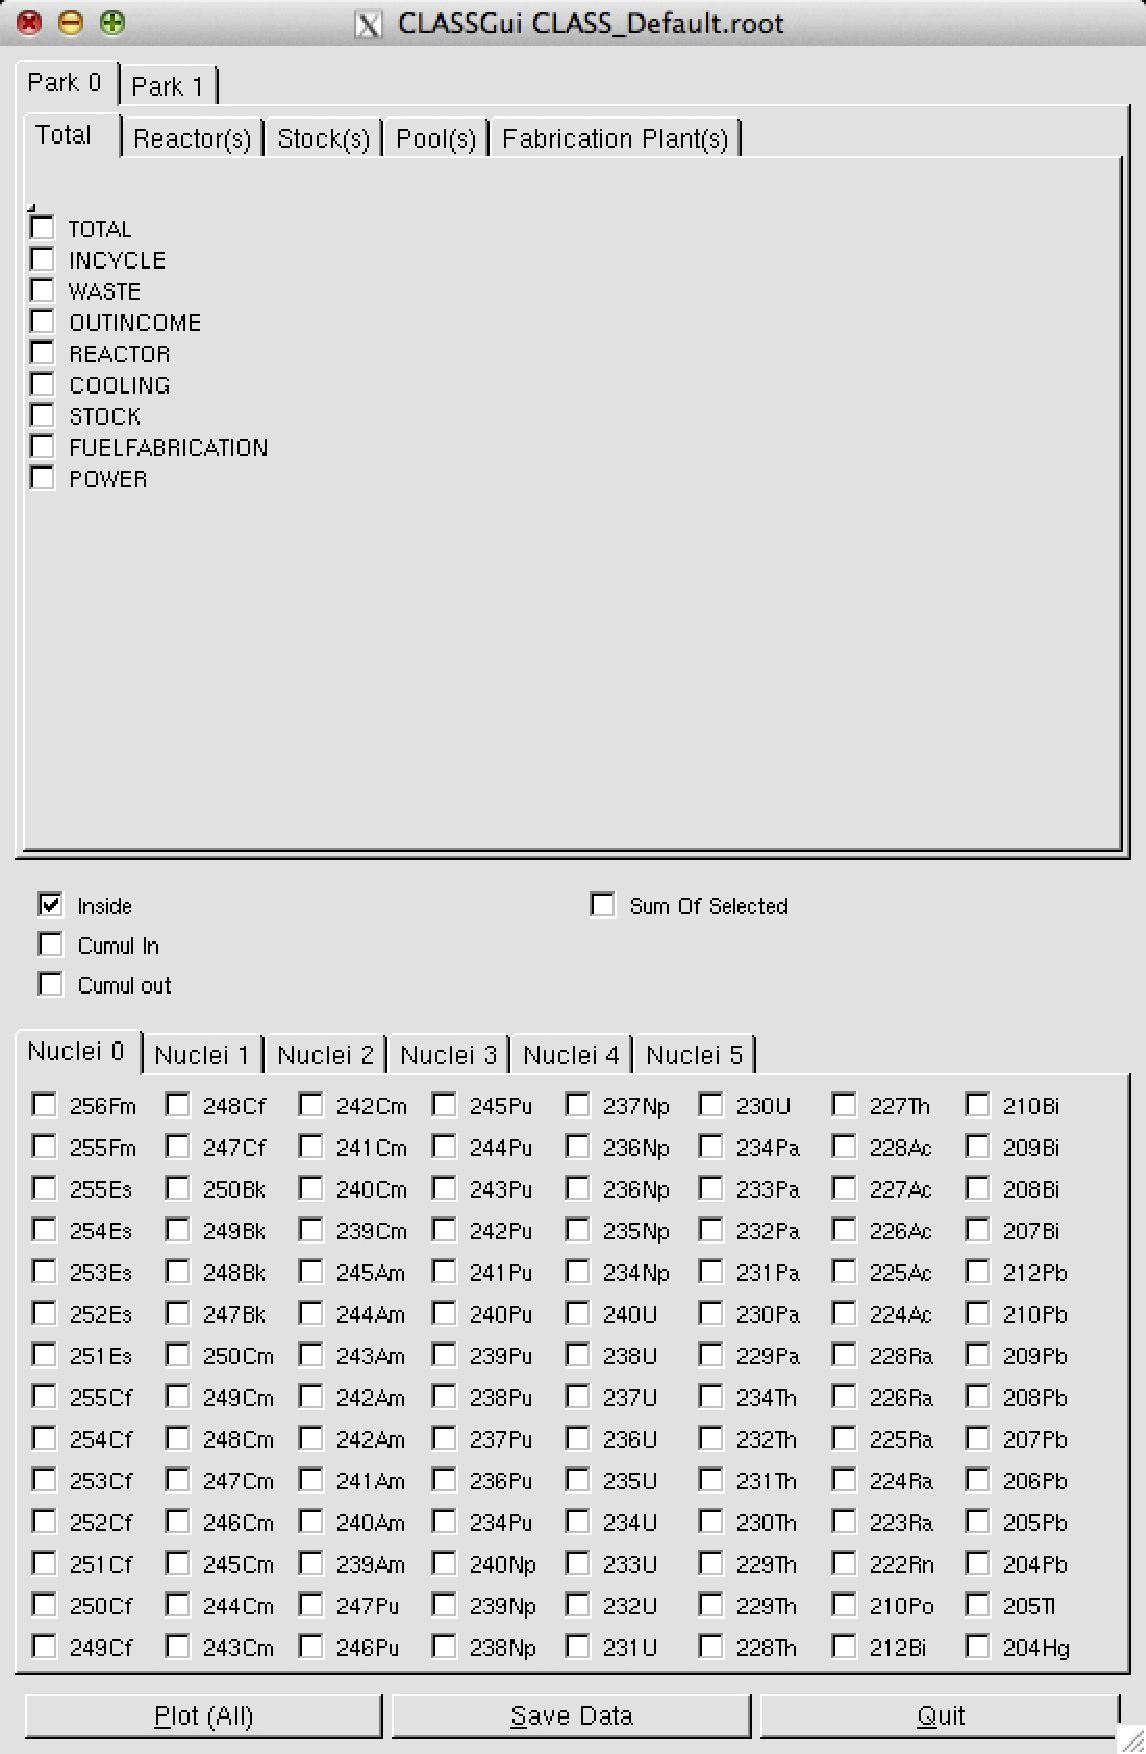
\includegraphics[width=0.7\textwidth]{CLASSGui} 
\caption{The graphical user interface for CLASS outputs\label{fig:CLASSGui} }
\end{figure}





%%%%%%%%%%%%%%%%%%%%%%%%%
%% CHAPTER :	INPUT EXAMPLE
%%%%%%%%%%%%%%%%%%%%%%%%%
%\part{Input examples}




%%%%%%%%%%%%%%%%%%%%%%%%%
%% CHAPTER :	IN DEVELOPMENT
%%%%%%%%%%%%%%%%%%%%%%%%%
%\part{In development}



% === main matter ===
%\mainmatter
%\linenumbers
%\part{Recherche de la Vibration G\'eante de Paires}
%\include{ithemba_chapter_1_intro}
%\include{ithemba_chapter_2_des_exp}
%\include{ithemba_chapter_3_analyse}
%\include{ithemba_chapter_4_crosssection}
%\include{ithemba_chapter_5_discussion}
%\part{Mesure du temps de vie du premier �tat excit� $2^{+}$ du $^{74}$Zn par m\'ethode plunger.}
\bibliographystyle{wmaainf}
\bibliography{Biblio}

\end{document}
